\documentclass[]{book}
\usepackage{lmodern}
\usepackage{amssymb,amsmath}
\usepackage{ifxetex,ifluatex}
\usepackage{fixltx2e} % provides \textsubscript
\ifnum 0\ifxetex 1\fi\ifluatex 1\fi=0 % if pdftex
  \usepackage[T1]{fontenc}
  \usepackage[utf8]{inputenc}
\else % if luatex or xelatex
  \ifxetex
    \usepackage{mathspec}
  \else
    \usepackage{fontspec}
  \fi
  \defaultfontfeatures{Ligatures=TeX,Scale=MatchLowercase}
\fi
% use upquote if available, for straight quotes in verbatim environments
\IfFileExists{upquote.sty}{\usepackage{upquote}}{}
% use microtype if available
\IfFileExists{microtype.sty}{%
\usepackage{microtype}
\UseMicrotypeSet[protrusion]{basicmath} % disable protrusion for tt fonts
}{}
\usepackage[margin=1in]{geometry}
\usepackage{hyperref}
\hypersetup{unicode=true,
            pdftitle={The EMU-SDMS Manual},
            pdfborder={0 0 0},
            breaklinks=true}
\urlstyle{same}  % don't use monospace font for urls
\usepackage{natbib}
\bibliographystyle{apalike}
\usepackage{color}
\usepackage{fancyvrb}
\newcommand{\VerbBar}{|}
\newcommand{\VERB}{\Verb[commandchars=\\\{\}]}
\DefineVerbatimEnvironment{Highlighting}{Verbatim}{commandchars=\\\{\}}
% Add ',fontsize=\small' for more characters per line
\usepackage{framed}
\definecolor{shadecolor}{RGB}{248,248,248}
\newenvironment{Shaded}{\begin{snugshade}}{\end{snugshade}}
\newcommand{\KeywordTok}[1]{\textcolor[rgb]{0.13,0.29,0.53}{\textbf{{#1}}}}
\newcommand{\DataTypeTok}[1]{\textcolor[rgb]{0.13,0.29,0.53}{{#1}}}
\newcommand{\DecValTok}[1]{\textcolor[rgb]{0.00,0.00,0.81}{{#1}}}
\newcommand{\BaseNTok}[1]{\textcolor[rgb]{0.00,0.00,0.81}{{#1}}}
\newcommand{\FloatTok}[1]{\textcolor[rgb]{0.00,0.00,0.81}{{#1}}}
\newcommand{\ConstantTok}[1]{\textcolor[rgb]{0.00,0.00,0.00}{{#1}}}
\newcommand{\CharTok}[1]{\textcolor[rgb]{0.31,0.60,0.02}{{#1}}}
\newcommand{\SpecialCharTok}[1]{\textcolor[rgb]{0.00,0.00,0.00}{{#1}}}
\newcommand{\StringTok}[1]{\textcolor[rgb]{0.31,0.60,0.02}{{#1}}}
\newcommand{\VerbatimStringTok}[1]{\textcolor[rgb]{0.31,0.60,0.02}{{#1}}}
\newcommand{\SpecialStringTok}[1]{\textcolor[rgb]{0.31,0.60,0.02}{{#1}}}
\newcommand{\ImportTok}[1]{{#1}}
\newcommand{\CommentTok}[1]{\textcolor[rgb]{0.56,0.35,0.01}{\textit{{#1}}}}
\newcommand{\DocumentationTok}[1]{\textcolor[rgb]{0.56,0.35,0.01}{\textbf{\textit{{#1}}}}}
\newcommand{\AnnotationTok}[1]{\textcolor[rgb]{0.56,0.35,0.01}{\textbf{\textit{{#1}}}}}
\newcommand{\CommentVarTok}[1]{\textcolor[rgb]{0.56,0.35,0.01}{\textbf{\textit{{#1}}}}}
\newcommand{\OtherTok}[1]{\textcolor[rgb]{0.56,0.35,0.01}{{#1}}}
\newcommand{\FunctionTok}[1]{\textcolor[rgb]{0.00,0.00,0.00}{{#1}}}
\newcommand{\VariableTok}[1]{\textcolor[rgb]{0.00,0.00,0.00}{{#1}}}
\newcommand{\ControlFlowTok}[1]{\textcolor[rgb]{0.13,0.29,0.53}{\textbf{{#1}}}}
\newcommand{\OperatorTok}[1]{\textcolor[rgb]{0.81,0.36,0.00}{\textbf{{#1}}}}
\newcommand{\BuiltInTok}[1]{{#1}}
\newcommand{\ExtensionTok}[1]{{#1}}
\newcommand{\PreprocessorTok}[1]{\textcolor[rgb]{0.56,0.35,0.01}{\textit{{#1}}}}
\newcommand{\AttributeTok}[1]{\textcolor[rgb]{0.77,0.63,0.00}{{#1}}}
\newcommand{\RegionMarkerTok}[1]{{#1}}
\newcommand{\InformationTok}[1]{\textcolor[rgb]{0.56,0.35,0.01}{\textbf{\textit{{#1}}}}}
\newcommand{\WarningTok}[1]{\textcolor[rgb]{0.56,0.35,0.01}{\textbf{\textit{{#1}}}}}
\newcommand{\AlertTok}[1]{\textcolor[rgb]{0.94,0.16,0.16}{{#1}}}
\newcommand{\ErrorTok}[1]{\textcolor[rgb]{0.64,0.00,0.00}{\textbf{{#1}}}}
\newcommand{\NormalTok}[1]{{#1}}
\usepackage{longtable,booktabs}
\usepackage{graphicx,grffile}
\makeatletter
\def\maxwidth{\ifdim\Gin@nat@width>\linewidth\linewidth\else\Gin@nat@width\fi}
\def\maxheight{\ifdim\Gin@nat@height>\textheight\textheight\else\Gin@nat@height\fi}
\makeatother
% Scale images if necessary, so that they will not overflow the page
% margins by default, and it is still possible to overwrite the defaults
% using explicit options in \includegraphics[width, height, ...]{}
\setkeys{Gin}{width=\maxwidth,height=\maxheight,keepaspectratio}
\IfFileExists{parskip.sty}{%
\usepackage{parskip}
}{% else
\setlength{\parindent}{0pt}
\setlength{\parskip}{6pt plus 2pt minus 1pt}
}
\setlength{\emergencystretch}{3em}  % prevent overfull lines
\providecommand{\tightlist}{%
  \setlength{\itemsep}{0pt}\setlength{\parskip}{0pt}}
\setcounter{secnumdepth}{5}
% Redefines (sub)paragraphs to behave more like sections
\ifx\paragraph\undefined\else
\let\oldparagraph\paragraph
\renewcommand{\paragraph}[1]{\oldparagraph{#1}\mbox{}}
\fi
\ifx\subparagraph\undefined\else
\let\oldsubparagraph\subparagraph
\renewcommand{\subparagraph}[1]{\oldsubparagraph{#1}\mbox{}}
\fi

%%% Use protect on footnotes to avoid problems with footnotes in titles
\let\rmarkdownfootnote\footnote%
\def\footnote{\protect\rmarkdownfootnote}

%%% Change title format to be more compact
\usepackage{titling}

% Create subtitle command for use in maketitle
\newcommand{\subtitle}[1]{
  \posttitle{
    \begin{center}\large#1\end{center}
    }
}

\setlength{\droptitle}{-2em}
  \title{The EMU-SDMS Manual}
  \pretitle{\vspace{\droptitle}\centering\huge}
  \posttitle{\par}
  \author{}
  \preauthor{}\postauthor{}
  \predate{\centering\large\emph}
  \postdate{\par}
  \date{2017-10-09}

\usepackage{booktabs}
\usepackage{amsthm}
\makeatletter
\def\thm@space@setup{%
  \thm@preskip=8pt plus 2pt minus 4pt
  \thm@postskip=\thm@preskip
}
\makeatother

\usepackage{amsthm}
\newtheorem{theorem}{Theorem}[chapter]
\newtheorem{lemma}{Lemma}[chapter]
\theoremstyle{definition}
\newtheorem{definition}{Definition}[chapter]
\newtheorem{corollary}{Corollary}[chapter]
\newtheorem{proposition}{Proposition}[chapter]
\theoremstyle{definition}
\newtheorem{example}{Example}[chapter]
\theoremstyle{definition}
\newtheorem{exercise}{Exercise}[chapter]
\theoremstyle{remark}
\newtheorem*{remark}{Remark}
\newtheorem*{solution}{Solution}
\begin{document}
\maketitle

{
\setcounter{tocdepth}{1}
\tableofcontents
}
\chapter{Installing the EMU-SDMS}\label{installing-the-emu-sdms}

\begin{enumerate}
\def\labelenumi{\arabic{enumi}.}
\tightlist
\item
  \texttt{R}
\end{enumerate}

\begin{itemize}
\tightlist
\item
  Download the R programming language from
  \href{www.cran.r-project.org}{http://www.cran.r-project.org}
\item
  Install the R programming language by executing the downloaded file
  and following the on-screen instructions.
\end{itemize}

\begin{enumerate}
\def\labelenumi{\arabic{enumi}.}
\setcounter{enumi}{1}
\tightlist
\item
  \texttt{emuR}
\end{enumerate}

\begin{itemize}
\tightlist
\item
  Start up R.
\item
  Enter \texttt{install.packages("emuR")} after the
  \texttt{\textgreater{}} prompt to install the package. (You will only
  need to repeat this if package updates become available.)
\item
  As the \texttt{wrassp} package is a dependency of the \texttt{emuR}
  package, it does not have to be installed separately.
\end{itemize}

\begin{enumerate}
\def\labelenumi{\arabic{enumi}.}
\setcounter{enumi}{2}
\tightlist
\item
  \texttt{EMU-webApp} (prerequisite)
\end{enumerate}

\begin{itemize}
\tightlist
\item
  The only thing needed to use the \texttt{EMU-webApp} is a current
  HTML5 compatible browser (Chrome/Firefox/Safari/Opera/\ldots{}).
  However, as most of the development and testing is done using Chrome
  we recommend using it, as it is by far the best tested browser.
\end{itemize}

\section{Installing additional R-packages that are used throughout this
document}\label{installing-additional-r-packages-that-are-used-throughout-this-document}

\begin{itemize}
\tightlist
\item
  \texttt{ggplot2} for visualization purposes:
  \texttt{install.packages("emuR")}
\item
  \texttt{dplyr} for data manipulation:
  \texttt{install.packages("dplyr")}
\end{itemize}

\section{Version disclaimer}\label{version-disclaimer}

This document describes the following versions of the software
components:

\begin{itemize}
\tightlist
\item
  \texttt{wrassp}

  \begin{itemize}
  \tightlist
  \item
    Package version: 0.1.4
  \item
    Git SHA1:
    \texttt{jsonlite::fromJSON("https://api.github.com/repos/IPS-LMU/wrassp/branches/master")\$commit\$sha}
  \end{itemize}
\item
  \texttt{emuR}

  \begin{itemize}
  \tightlist
  \item
    Package version: \texttt{packageVersion("emuR")}
  \item
    Git SHA1:
    \texttt{jsonlite::fromJSON("https://api.github.com/repos/IPS-LMU/emuR/branches/master")\$commit\$sha}
  \end{itemize}
\item
  \texttt{EMU-webApp}

  \begin{itemize}
  \tightlist
  \item
    Version:
    \texttt{jsonlite::fromJSON("https://raw.githubusercontent.com/IPS-LMU/EMU-webApp/master/package.json")\$version}
  \item
    Git SHA1:
    \texttt{jsonlite::fromJSON("https://api.github.com/repos/IPS-LMU/EMU-webapp/branches/master")\$commit\$sha}
  \end{itemize}
\end{itemize}

As the development of the EMU Speech Database Management System is still
ongoing, be sure you have the correct documentation to go with the
version you are using.

\section{For developers and people interested in the source
code}\label{for-developers-and-people-interested-in-the-source-code}

The information on how to install and/or access the source code of the
developer version including the possibility of accessing the versions
described in this document (via the Git SHA1 hashes mentioned above) is
given below.

\begin{itemize}
\tightlist
\item
  \texttt{wrassp}

  \begin{itemize}
  \tightlist
  \item
    Source code is available here:
    \url{https://github.com/IPS-LMU/wrassp/}
  \item
    Install developer version in R:
    \texttt{install.packages("devtools");\ library("devtools");\ install\_github("IPS-LMU/wrassp")}
  \item
    Bug reports: \url{https://github.com/IPS-LMU/wrassp/issues}
  \end{itemize}
\item
  \texttt{emuR}

  \begin{itemize}
  \tightlist
  \item
    Source code is available here:
    \url{https://github.com/IPS-LMU/emuR/}
  \item
    Install developer version in R:
    \texttt{install.packages("devtools");\ library("devtools");\ install\_github("IPS-LMU/emuR")}
  \item
    Bug reports: \url{https://github.com/IPS-LMU/emuR/issues}
  \end{itemize}
\item
  \texttt{EMU-webApp}

  \begin{itemize}
  \tightlist
  \item
    Source code is available here:
    \url{https://github.com/IPS-LMU/EMU-webApp/}
  \item
    Bug reports: \url{https://github.com/IPS-LMU/EMU-webApp/issues}
  \end{itemize}
\end{itemize}

\chapter[An overview of the EMU-SDMS ]{\texorpdfstring{An overview of
the EMU-SDMS \footnote{Sections of this chapter have been published in
  \citet{winkelmann:2017aa}}}{An overview of the EMU-SDMS }}\label{chap:overview}


\includegraphics[width=14.22in]{pics/EMU-webAppIcon-roundCorners}

The EMU Speech Database Management System is a collection of software
tools which aims to be as close to an all-in-one solution for
generating, manipulating, querying, analyzing and managing speech
databases as possible. It was developed to fill the void in the
landscape of software tools for the speech sciences by providing an
integrated system that is centered around the R language and environment
for statistical computing and graphics \citep{r-core-team:2016a}. This
manual contains the documentation for the three software components
\texttt{wrassp}, \texttt{emuR} and the \texttt{EMU-webApp}. In addition,
it provides an in-depth description of the \texttt{emuDB} database
format which is also considered an integral part of the new system.
These four components comprise the EMU-SDMS and benefit the speech
sciences and spoken language research by providing an integrated system
to answer research questions such as: \emph{Given an annotated speech
database, is vowel height (measured by its correlate, the first formant
frequency) influenced by whether it appears in a strong or weak
syllable?}

This manual is targeted at new EMU-SDMS users as well as users familiar
with the legacy EMU system. In addition, it is aimed at people who are
interested in the technical details such as data structures/formats and
implementation strategies, be it for reimplementation purposes or simply
for a better understanding of the inner workings of the new system. To
accommodate these different target groups, after initially giving an
overview of the system, this manual presents a usage tutorial that walks
the user through the entire process of answering a research question.
This tutorial will start with a set of \texttt{.wav} audio and Praat
\texttt{.TextGrid} \citep{boersma:2011a} annotation files and end with a
statistical analysis to address the hypothesis posed by the research
question. The following Part \ref{part:mainCompAndConc} of this
documentation is separated into six chapters that give an in-depth
explanation of the various components that comprise the EMU-SDMS and
integral concepts of the new system. These chapters provide a
tutorial-like overview by providing multiple examples. To give the
reader a synopsis of the main functions and central objects that are
provided by EMU-SDMS's main R package \texttt{emuR}, an overview of
these functions is presented in Part \ref{part:emuRfuncs}. Part
\ref{part:impl} focuses on the actual implementation of the components
and is geared towards people interested in the technical details.
Further examples and file format descriptions are available in various
appendices. This structure enables the novice EMU-SDMS user to simply
skip the technical details and still get an in-depth overview of how to
work with the new system and discover what it is capable of.

A prerequisite that is presumed throughout this document is the reader's
familiarity with basic terminology in the speech sciences (e.g.,
familiarity with the international phonetic alphabet (IPA) and how
speech is annotated at a coarse and fine grained level). Further, we
assume the reader has a grasp of the basic concepts of the R language
and environment for statistical computing and graphics. For readers new
to R, there are multiple, freely available R tutorials online (e.g.,
\url{https://en.wikibooks.org/wiki/Statistical_Analysis:_an_Introduction_using_R/R_basics}.
R also has a set of very detailed manuals and tutorials that come
preinstalled with R. To be able to access R's own ``An Introduction to
R'' introduction, simply type \texttt{help.start()} into the R console
and click on the link to the tutorial.

\section{The evolution of the
EMU-SDMS}\label{the-evolution-of-the-emu-sdms}

The EMU-SDMS has a number of predecessors that have been continuously
developed over a number of years \citep[e.g.,][\citet{cassidy:1996a},
\citet{cassidy:sc2001a}, \citet{bombien:2006a},
\citet{harrington:2010a}, \citet{john:2012a}]{harrington:csl1993a}. The
components presented here are the completely rewritten and newly
designed, next incarnation of the EMU system, which we will refer to as
the EMU Speech Database Management System (EMU-SDMS). The EMU-SDMS keeps
most of the core concepts of the previous system, which we will refer to
as the legacy system, in place while improving on things like usability,
maintainability, scalability, stability, speed and more. We feel the
redesign and reimplementation elevates the system into a modern set of
speech and language tools that enables a workflow adapted to the
challenges confronting speech scientists and the ever growing size of
speech databases. The redesign has enabled us to implement several
components of the new EMU-SDMS so that they can be used independently of
the EMU-SDMS for tasks such as web-based collaborative annotation
efforts and performing speech signal processing in a statistical
programming environment. Nevertheless, the main goal of the redesign and
reimplementation was to provide a modern set of tools that reduces the
complexity of the tool chain needed to answer spoken language research
questions down to a few interoperable tools. The tools the EMU-SDMS
provides are designed to streamline the process of obtaining usable
data, all from within an environment that can also be used to analyze,
visualize and statistically evaluate the data.

Upon developing the new system, rather than starting completely from
scratch it seemed more appropriate to partially reuse the concepts of
the legacy system in order to achieve our goals. A major observation at
the time was that the R language and environment for statistical
computing and graphics \citep{r-core-team:2016a} was gaining more and
more traction for statistical and data visualization purposes in the
speech and spoken language research community. However, R was mostly
only used towards the end of the data analysis chain where data usually
was pre-converted into a comma-separated values or equivalent file
format by the user using other tools to calculate, extract and
pre-process the data. While designing the new EMU-SDMS, we brought R to
the front of the tool chain to the point just beyond data acquisition.
This allows the entire data annotation, data extraction and analysis
process to be completed in R, while keeping the key user requirements in
mind. Due to the personal experiences gained by using the legacy system
in various undergraduate courses \citep[course material usually based
on][]{harrington:2010a}, we learned that the key user requirements were
data and database portability, a simple installation process, an as
pleasant as possible user experience and cross-platform availability.
Supplying all of EMU-SDMS's core functionality in the form of R packages
that do not rely on external software at runtime seemed to meet all of
these requirements.

As the early incarnations of the legacy EMU system and its predecessors
were conceived either at a time that predated the R system or during the
infancy of R's package ecosystem, the legacy system was implemented as a
modular yet composite standalone program with a communication and data
exchange interface to the R/Splus systems \citep[see][ Section 3 for
details]{cassidy:sc2001a}. Recent developments in the package ecosystem
of R such as the availability of the \texttt{DBI} package
\citep{r-special-interest-group-on-databases-r-sig-db:2016a} and the
related packages \texttt{RSQLite} and \texttt{RPostgreSQL}
\citep[\citet{conway:2016a}]{wickham:2014a}, as well as the
\texttt{jsonlite} package \citep{ooms:as2014a} and the \texttt{httpuv}
package \citep{rstudio:2015a}, have made R an attractive sole target
platform for the EMU-SDMS. These and other packages provide additional
functional power that enabled the EMU-SDMS's core functionality to be
implemented in the form of R packages. The availability of certain R
packages had a large impact on the architectural design decisions that
we made for the new system.

R Example @ref(rexample:overview\_install) shows the simple installation
process which we were able to achieve due to the R package
infrastructure. Compared to the legacy EMU and other systems, the
installation process of the entire system has been reduced to a single R
command. Throughout this documentation we will try to highlight how the
EMU-SDMS is also able to meet the rest of the above key user
requirements.

\begin{Shaded}
\begin{Highlighting}[]
\CommentTok{# install the entire EMU-SDMS}
\CommentTok{# by installing the emuR package}
\KeywordTok{install.packages}\NormalTok{(}\StringTok{"emuR"}\NormalTok{)}
\end{Highlighting}
\end{Shaded}

It is worth noting that throughout this manual R Example code snippets
will be given in the form of R Example @ref(rexample:overview\_install).
These examples represent working R code that allow the reader to follow
along in a hands-on manor and give a feel for what it is like working
with the new EMU-SDMS.

\section{EMU-SDMS: System architecture and default
workflow}\label{emu-sdms-system-architecture-and-default-workflow}

\label{sec:overview_sysArch}

As was previously mentioned, the new EMU-SDMS is made up of four main
components. The components are the \texttt{emuDB} format; the R packages
\texttt{wrassp} and \texttt{emuR}; and the web application, the
\texttt{EMU-webApp}, which is EMU-SDMS's new graphical user interface
(GUI) component. An overview of the EMU-SDMS's architecture and the
components' relationships within the system is shown in Figure
@ref(fig:overview\_archOver). In Figure @ref(fig:overview\_archOver),
the \texttt{emuR} package plays a central role as it is the only
component that interacts with all of the other components of the
EMU-SDMS. It performs file and DB handling for the files that comprise
an \texttt{emuDB} (see Chapter @ref(chap:annot\_struct\_mod)); it uses
the \texttt{wrassp} package for signal processing purposes (see Chapter
\ref{chap:wrassp}); and it can serve \texttt{emuDB}s to the
\texttt{EMU-webApp} (see Chapter \ref{chap:emu-webApp}).

\begin{figure}
\centering
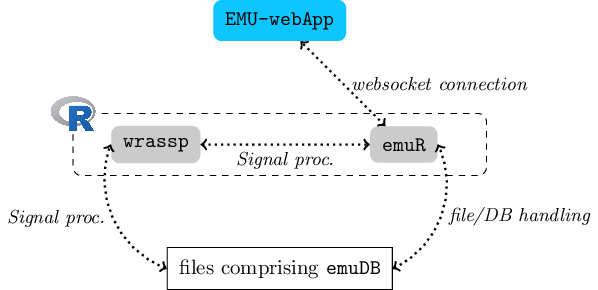
\includegraphics{pics/overview.png}
\caption{Schematic architecture of the
EMU-SDMS.(\#fig:overview\_archOver)}
\end{figure}

Although the system is made of four main components, the user largely
only interacts directly with the \texttt{EMU-webApp} and the
\texttt{emuR} package. A summary of the default workflow illustrating
theses interactions can be seen below:

\begin{enumerate}
\def\labelenumi{\arabic{enumi}.}
\tightlist
\item
  Load database into current R session (\texttt{load\_emuDB()}).
\item
  Database annotation / visual inspection (\texttt{serve()}). This opens
  up the \texttt{EMU-webApp} in the system's default browser.
\item
  Query database (\texttt{query()}). This is optionally followed by
  \texttt{requery\_hier()} or \texttt{requery\_seq()} as necessary (see
  Chapter \ref{chap:querysys} for details).
\item
  Get trackdata (e.g.~formant values) for the result of a query
  (\texttt{get\_trackdata()}).
\item
  Prepare data.
\item
  Visually inspect data.
\item
  Carry out further analysis and statistical processing.
\end{enumerate}

Initially the user creates a reference to an \texttt{emuDB} by loading
it into their current R session using the \texttt{load\_emuDB()}
function (see step 1). This database reference can then be used to
either serve (\texttt{serve()}) the database to the \texttt{EMU-webApp}
or query (\texttt{query()}) the annotations of the \texttt{emuDB} (see
steps 2 and 3). The result of a query can then be used to either perform
one or more so-called requeries or extract signal values that correspond
to the result of a \texttt{query()} or \texttt{requery()} (see step 4).
Finally, the signal data can undergo further preparation (e.g.,
correction of outliers) and visual inspection before further analysis
and statistical processing is carried out (see steps 5, 6 and 7).
Although the R packages provided by the EMU-SDMS do provide functions
for steps 4, 5 and 6, it is worth noting that the plethora of R packages
that the R package ecosystem provides can and should be used to perform
these duties. The resulting objects of most of the above functions are
derived \texttt{matrix} or \texttt{data.frame} objects which can be used
as inputs for hundreds if not thousands of other R functions.

\section{EMU-SDMS: Is it something for
you?}\label{emu-sdms-is-it-something-for-you}

\label{sec:overview_unique}

Besides providing a fully integrated system, the EMU-SDMS has several
unique features that set it apart from other current, widely used
systems \citep[e.g.,][\citet{wittenburg:2006a}, \citet{fromont:2012a},
\citet{rose:2006a}, \citet{mcauliffe:2016a}]{boersma:2011a}. To our
knowledge, the EMU-SDMS is the only system that allows the user to model
their annotation structures based on a hybrid model of time-based
annotations (such as those offered by Praat's tier-based annotation
mechanics) and hierarchical timeless annotations. An example of such a
hybrid annotation structure is displayed in Figure
@ref(overview\_hybridAnnot). These hybrid annotations benefit the user
in multiple ways, as they reduce data redundancy and explicitly allow
relationships to be expressed across annotation levels (see Chapter
@ref(chap:annot\_struct\_mod) for further information on hierarchical
annotations and Chapter \ref{chap:querysys} on how to query these
annotation structures).

\begin{figure}
\centering
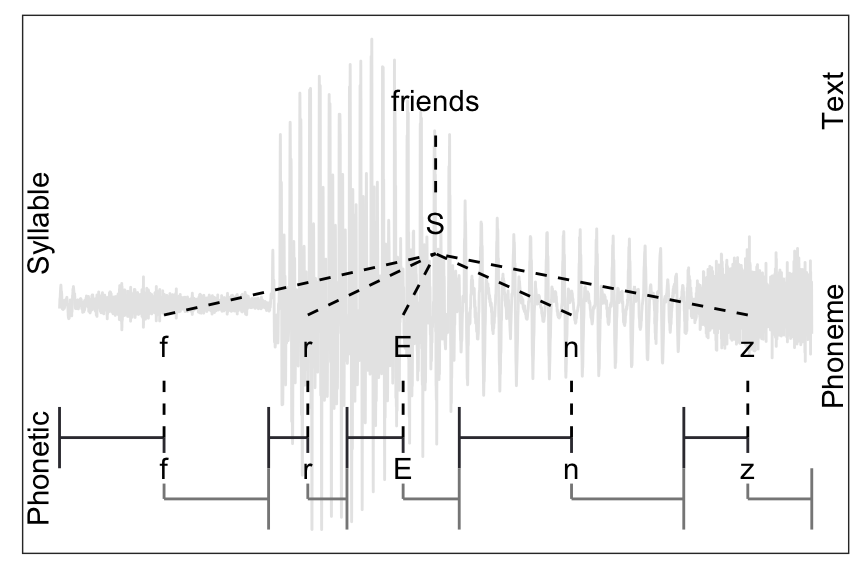
\includegraphics{The-EMU-SDMS-Manual_files/figure-latex/overview_hybridAnnot-1.pdf}
\caption{(\#fig:overview\_hybridAnnot)Example of a hybrid annotation
combining time-based (\emph{Phonetic} level) and hierarchical
(\emph{Phoneme}, \emph{Syllable}, \emph{Text} levels including the
inter-level links) annotations.}
\end{figure}

Further, to our knowledge, the EMU-SDMS is the first system that makes
use of a web application as its primary GUI for annotating speech. This
unique approach enables the GUI component to be used in multiple ways.
It can be used as a stand-alone annotation tool, connected to a loaded
\texttt{emuDB} via \texttt{emuR}'s \texttt{serve()} function and used to
communicate to other servers. This enables it to be used as a
collaborative annotation tool. An in-depth explanation of how this
component can be used in these three scenarios is given in Chapter
\ref{chap:emu-webApp}.

As demonstrated in the default workflow of Section
@ref(sec:overview\_sysArch), an additional unique feature provided by
EMU-SDMS is the ability use the result of a query to extract derived
(e.g., formants and RMS values) and complementary signals (e.g.,
electromagnetic articulography data) that match the segments of a query.
This, for example, aids the user in answering questions related to
derived speech signals such as: \emph{Is vowel height (measured by its
correlate, the first formant frequency) influenced by whether it appears
in a strong or weak syllable?}. Chapter \ref{chap:tutorial} gives a
complete walk-through of how to go about answering this question using
the tools provided by the EMU-SDMS.

The features provided by the EMU-SDMS make it an all-in-one speech
database management solution that is centered around R. It enriches the
R platform by providing specialized speech signal processing, speech
database management, data extraction and speech annotation capabilities.
By achieving this without relying on any external software sources
except the web browser, the EMU-SDMS significantly reduces the number of
tools the speech and spoken language researcher has to deal with and
helps to simplify answering research questions. As the only prerequisite
for using the EMU-SDMS is a basic familiarity with the R platform, if
the above features would improve your workflow, the EMU-SDMS is indeed
for you.

\chapter[A tutorial on how to use the EMU-SDMS ]{\texorpdfstring{A
tutorial on how to use the EMU-SDMS \footnote{Some examples of this
  chapter are adapted versions of examples of the \texttt{emuR\_intro}
  vignette.}}{A tutorial on how to use the EMU-SDMS }}\label{chap:tutorial}

\begin{figure}
\centering
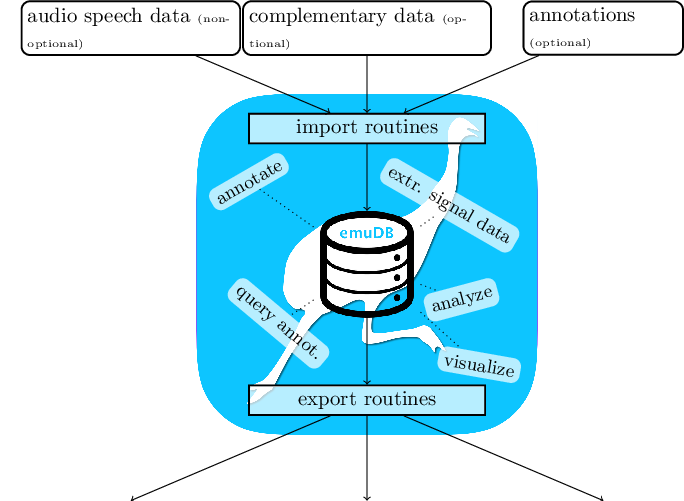
\includegraphics{pics/emuSdmsBirdsEye.png}
\caption{}
\end{figure}

Using the tools provided by the EMU-SDMS, this tutorial chapter gives a
practical step-by-step guide to answering the question: \emph{Given an
annotated speech database, is vowel height (measured by its correlate,
the first formant frequency) influenced by whether it appears in a
strong or weak syllable?} The tutorial only skims over many of the
concepts and functions provided by the EMU-SDMS. In-depth explanations
of the various functionalities are given in later chapters of this
documentation.

As the EMU-SDMS is not concerned with the raw data acquisition, other
tools such as SpeechRecorder by \citet{draxler:2004a} are first used to
record speech. However, once audio speech recordings are available, the
system provides multiple conversion routines for converting existing
collections of files to the new \texttt{emuDB} format described in
Chapter \ref{chap:emuDB} and importing them into the new EMU system. The
current import routines provided by the \texttt{emuDB} package are:

\begin{itemize}
\tightlist
\item
  \texttt{convert\_TextGridCollection()} - Convert TextGrid collections
  (\texttt{.wav} and \texttt{.TextGrid} files) to the \texttt{emuDB}
  format,
\item
  \texttt{convert\_BPFCollection()} - Convert BPF collections
  (\texttt{.wav} and \texttt{.par}\} files) to the \texttt{emuDB}
  format,
\item
  \texttt{convert\_txtCollection()} - Convert plain text file
  collections format (\texttt{.wav} and \texttt{.txt} files) to the
  \texttt{emuDB} format,
\item
  \texttt{convert\_legacyEmuDB()} - Convert the legacy EMU database
  format to the \texttt{emuDB} format and
\item
  \texttt{create\_emuDB()} followed by
  \texttt{add\_link/levelDefinition} and \texttt{import\_mediaFiles()} -
  Creating \texttt{emuDB}s from scratch with only audio files present.
\end{itemize}

The \texttt{emuDB} package comes with a set of example files and small
databases that are used throughout the \texttt{emuDB} documentation,
including the functions help pages. These can be accessed by typing
\texttt{help(functionName)} or the short form \texttt{?functionName}. R
Example @ref(rexample:tutorial\_create\_emuRdemoData) illustrates how to
create this demo data in a user-specified directory. Throughout the
examples of this documentation the directory that is provided by the
base R function \texttt{tempdir()} will be used, as this is available on
every platform supported by R (see \texttt{?tempdir} for further
details). As can be inferred from the \texttt{list.dirs()} output in R
Example @ref(rexample:tutorial\_create\_emuRdemoData), the
\texttt{emuR\_demoData} directory contains a separate directory
containing example data for each of the import routines. Additionally,
it contains a directory containing an \texttt{emuDB} called \emph{ae}
(the directories name is \texttt{ae\_emuDB}, where \texttt{\_emuDB} is
the default suffix given to directories containing a \texttt{emuDB}; see
Chapter \ref{chap:emuDB}).

\begin{Shaded}
\begin{Highlighting}[]
\CommentTok{# load the package}
\KeywordTok{library}\NormalTok{(emuR)}

\CommentTok{# create demo data in directory provided by the tempdir() function}
\CommentTok{# (of course other directory paths may be chosen)}
\KeywordTok{create_emuRdemoData}\NormalTok{(}\DataTypeTok{dir =} \KeywordTok{tempdir}\NormalTok{())}

\CommentTok{# create path to demo data directory, which is}
\CommentTok{# called "emuR_demoData"}
\NormalTok{demoDataDir =}\StringTok{ }\KeywordTok{file.path}\NormalTok{(}\KeywordTok{tempdir}\NormalTok{(), }\StringTok{"emuR_demoData"}\NormalTok{)}

\CommentTok{# show demo data directories}
\KeywordTok{list.dirs}\NormalTok{(demoDataDir, }\DataTypeTok{recursive =} \NormalTok{F, }\DataTypeTok{full.names =} \NormalTok{F)}
\end{Highlighting}
\end{Shaded}

\begin{verbatim}
## [1] "ae_emuDB"            "BPF_collection"      "legacy_ae"          
## [4] "TextGrid_collection" "txt_collection"
\end{verbatim}

This tutorial will start by converting a TextGrid collection containing
seven annotated single-sentence utterances of a single male speaker to
the \texttt{emuDB} format\footnote{The other input routines are covered
  in the Section @ref(sec:emuRpackageDetails\_importRoutines).}. In the
EMU-SDMS, a file collection such as a TextGrid collection refers to a
set of file pairs where two types of files with different file
extentions are present (e.g., \texttt{.ext1} and \texttt{.ext2}). It is
vital that file pairs have the same basenames (e.g., \texttt{A.ext1} and
\texttt{A.ext2} where \texttt{A} represents the basename) in order for
the conversion functions to be able to pair up files that belong
together. As other speech software tools also encourage such file pairs
\citep[e.g.,][]{kisler:2015a} this is a common collection format in the
speech sciences. R Example \ref{rexample:showTGcolContent} shows such a
file collection that is part of \texttt{emuDB}'s demo data. Figure
@ref(fig:msajc003\_praatTG) shows the content of an annotation as
displayed by Praat's \texttt{"Draw\ visible\ sound\ and\ Textgrid..."}
procedure.

\begin{Shaded}
\begin{Highlighting}[]
\CommentTok{# create path to TextGrid collection}
\NormalTok{tgColDir =}\StringTok{ }\KeywordTok{file.path}\NormalTok{(demoDataDir, }\StringTok{"TextGrid_collection"}\NormalTok{)}

\CommentTok{# show content of TextGrid_collection directory}
\KeywordTok{list.files}\NormalTok{(tgColDir)}
\end{Highlighting}
\end{Shaded}

\begin{verbatim}
##  [1] "msajc003.TextGrid" "msajc003.wav"      "msajc010.TextGrid"
##  [4] "msajc010.wav"      "msajc012.TextGrid" "msajc012.wav"     
##  [7] "msajc015.TextGrid" "msajc015.wav"      "msajc022.TextGrid"
## [10] "msajc022.wav"      "msajc023.TextGrid" "msajc023.wav"     
## [13] "msajc057.TextGrid" "msajc057.wav"
\end{verbatim}

\begin{figure}
\centering
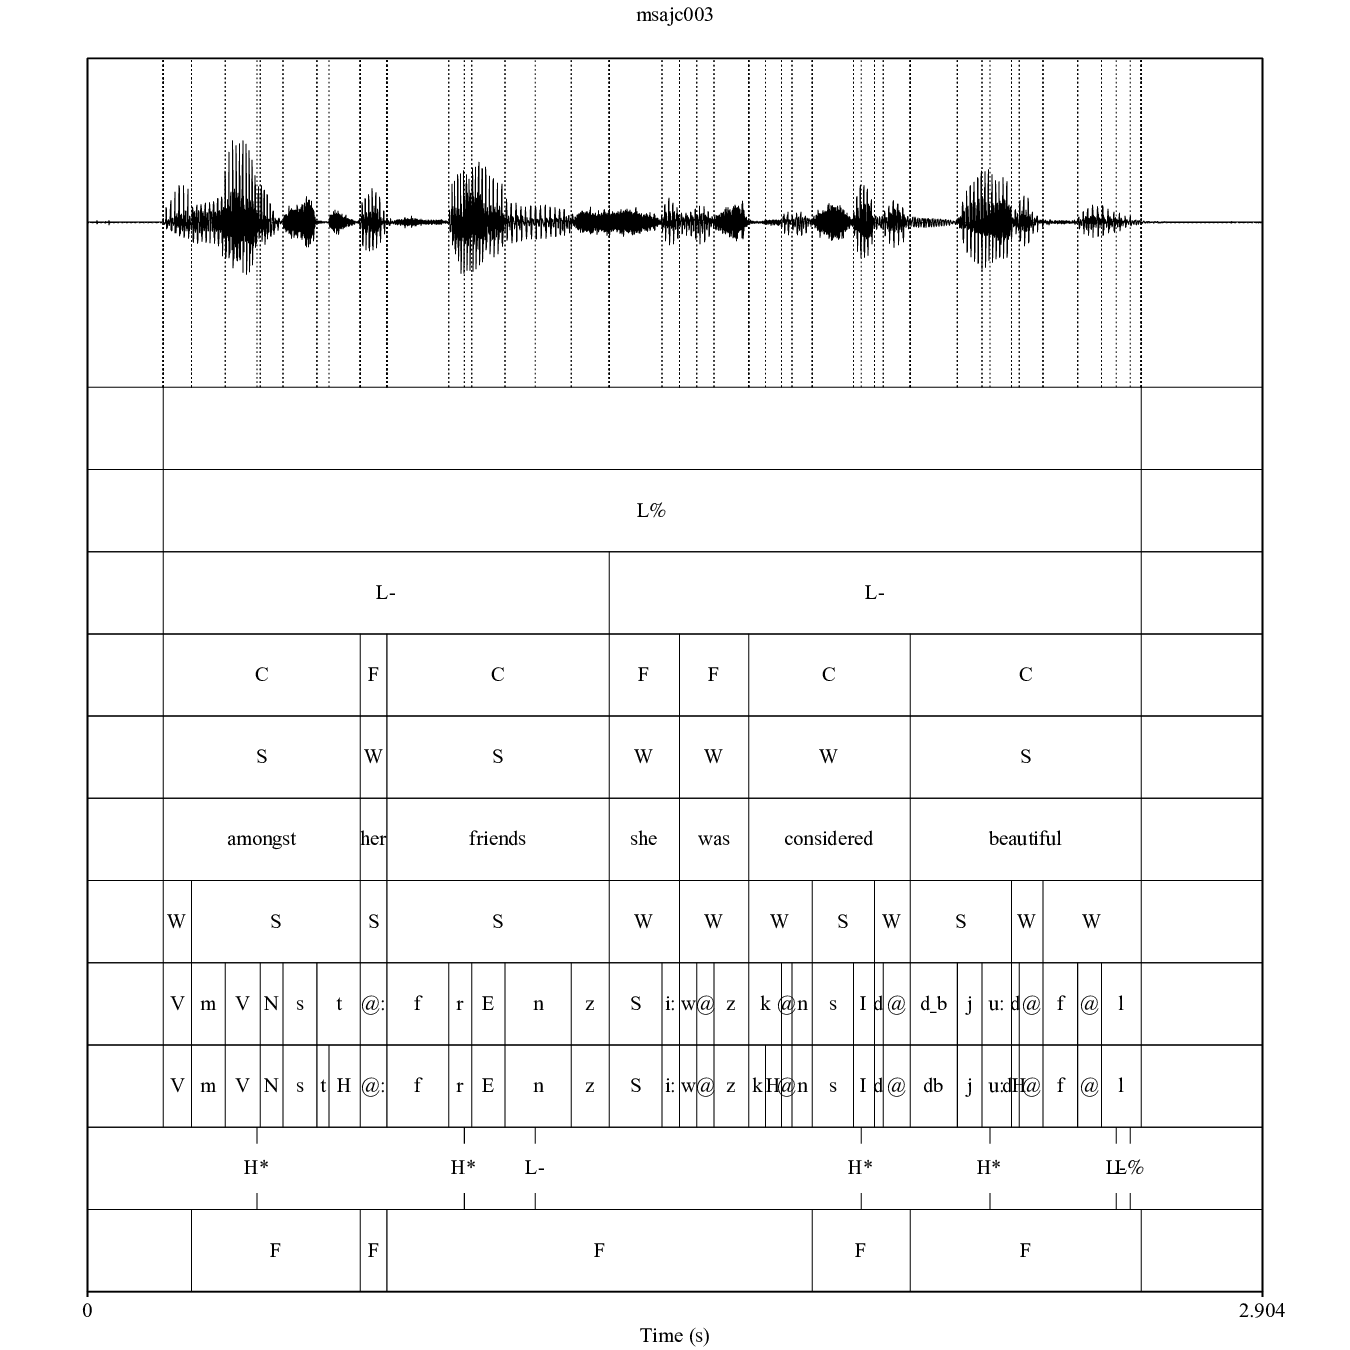
\includegraphics{pics/msajc003_praat.png}
\caption{TextGrid annotation of the
\texttt{emuR\_demoData/TextGrid\_collection/\textbackslash{}allowbreak\ msajc003.wav}
/ \texttt{.TextGrid} file pair containing the tiers (from top to
bottom): \emph{Utterance}, \emph{Intonational}, \emph{Intermediate},
\emph{Word}, \emph{Accent}, \emph{Text}, \emph{Syllable},
\emph{Phoneme}, \emph{Phonetic}, \emph{Tone},
\emph{Foot}.(\#fig:msajc003\_praatTG)}
\end{figure}

\section{Converting the TextGrid
collection}\label{converting-the-textgrid-collection}

The \texttt{convert\_TextGridCollection()} function converts a TextGrid
collection to the \texttt{emuDB} format. A precondition that all
\texttt{.TextGrid} files have to fulfill is that they must all contain
the same tiers. If this is not the case, yet there is an equal tier
subset that is contained in all the TextGrid files, this equal subset
may be chosen. For example, if all \texttt{.TextGrid} files contain only
the tier \texttt{Phonetic:\textbackslash{}\ IntervalTier} the conversion
will work. However, if a single \texttt{.TextGrid} of the collection has
the additional tier \texttt{Tone:\ TextTier} the conversion will fail.
In this case the conversion could be made to work by specifying the
equal subset (e.g., \texttt{equalSubset\ =\ c("Phonetic")}) and passing
it on to the \texttt{tierNames} function argument
\texttt{convert\_TextGridCollection(...,\ tierNames\ =\ equalSubset,\ ...)}.
As can be seen in Figure @ref(fig:msajc003\_praatTG), the TextGrid files
provided by the demo data contain eleven tiers. To reduce the complexity
of the annotations for this tutorial we will only convert the tiers
\emph{Text} (orthographic word annotations), \emph{Syllable} (strong:
\emph{S} vs.~weak: \emph{W} syllable annotations), \emph{Phoneme}
(phoneme level annotations) and \emph{Phonetic} (phonetic annotations)
utilizing the \texttt{tierNames} parameter. This conversion can be seen
in R Example @ref(rexample:tutorial\_tgconv).

\begin{Shaded}
\begin{Highlighting}[]
\CommentTok{# convert TextGrid collection to the emuDB format}
\KeywordTok{convert_TextGridCollection}\NormalTok{(}\DataTypeTok{dir =} \NormalTok{tgColDir,}
                           \DataTypeTok{dbName =} \StringTok{"myFirst"}\NormalTok{,}
                           \DataTypeTok{targetDir =} \KeywordTok{tempdir}\NormalTok{(),}
                           \DataTypeTok{tierNames =} \KeywordTok{c}\NormalTok{(}\StringTok{"Text"}\NormalTok{, }\StringTok{"Syllable"}\NormalTok{,}
                                         \StringTok{"Phoneme"}\NormalTok{, }\StringTok{"Phonetic"}\NormalTok{))}
\end{Highlighting}
\end{Shaded}

The above call to \texttt{convert\_TextGridCollection} creates a new
\texttt{emuDB} directory in the \texttt{tempdir()} directory called
\texttt{myFirst\_emuDB}. This \texttt{emuDB} contains annotation files
that contain the same \emph{Text}, \emph{Syllable}, \emph{Phoneme} and
\emph{Phonetic} segment tiers as the original \texttt{.TextGrid} files
as well as copies of the original (\texttt{.wav}) audio files. For
further details about the structure of an \texttt{emuDB}, see Chapter
\ref{chap:emuDB} of this document.

\section{Loading and inspecting the
database}\label{loading-and-inspecting-the-database}

As mentioned in Section @ref(sec:overview\_sysArch), the first step when
working with an \texttt{emuDB} is to load it into the current R session.
R Example @ref(rexample:tutorial\_loadEmuDB) shows how to load the
converted TextGrid collection into R using the \texttt{load\_emuDB()}
function.

\begin{Shaded}
\begin{Highlighting}[]
\CommentTok{# get path to emuDB called "myFirst"}
\CommentTok{# that was created by convert_TextGridCollection()}
\NormalTok{path2directory =}\StringTok{ }\KeywordTok{file.path}\NormalTok{(}\KeywordTok{tempdir}\NormalTok{(), }\StringTok{"myFirst_emuDB"}\NormalTok{)}

\CommentTok{# load emuDB into current R session}
\NormalTok{dbHandle =}\StringTok{ }\KeywordTok{load_emuDB}\NormalTok{(path2directory, }\DataTypeTok{verbose =} \OtherTok{FALSE}\NormalTok{)}
\end{Highlighting}
\end{Shaded}

\subsection{Overview}\label{overview}

Now the \emph{myFirst} \texttt{emuDB} is loaded into R, an overview of
the current status and configuration of the database can be displayed
using the \texttt{summary()} function as shown in R Example
@ref(rexample:tutorial\_summary).

\begin{Shaded}
\begin{Highlighting}[]
\CommentTok{# show summary}
\KeywordTok{summary}\NormalTok{(dbHandle)}
\end{Highlighting}
\end{Shaded}

\begin{verbatim}
## Name:     myFirst 
## UUID:     50e33f00-ae35-43d5-aa30-a84278c33a95 
## Directory:    /private/var/folders/ll/pw5k9y6x64q5xqys350rz2ph0000gn/T/RtmpAoRAeK/myFirst_emuDB 
## Session count: 1 
## Bundle count: 7 
## Annotation item count:  664 
## Label count:  664 
## Link count:  0 
## 
## Database configuration:
## 
## SSFF track definitions:
## NULL
## 
## Level definitions:
##       name    type nrOfAttrDefs attrDefNames
## 1     Text SEGMENT            1        Text;
## 2 Syllable SEGMENT            1    Syllable;
## 3  Phoneme SEGMENT            1     Phoneme;
## 4 Phonetic SEGMENT            1    Phonetic;
## 
## Link definitions:
## NULL
\end{verbatim}

The extensive output of \texttt{summary()} is split into a top and
bottom half, where the top half focuses on general information about the
database (name, directory, annotation item count, etc.) and the bottom
half displays information about the various Simple Signal File Format
(SSFF) track, level and link definitions of the \texttt{emuDB}. The
summary information about the level definitions shows, for instance,
that the \emph{myFirst} database has a \emph{Text} level of type
\texttt{SEGMENT} and therefore contains annotation items that have a
start time and a segment duration. It is worth noting that information
about the SSFF track, level and link definitions corresponds to the
output of the \texttt{list\_ssffTrackDefinitions()},
\texttt{list\_levelDefinitions()} and \texttt{list\_linkDefinitions()}
functions.

\subsection{Database annotation and visual
inspection}\label{database-annotation-and-visual-inspection}

The EMU-SDMS has a unique approach to annotating and visually inspecting
data-bases, as it utilizes a web application called the
\texttt{EMU-webApp} to act as its GUI. To be able to communicate with
the web application the \texttt{emuDB} package provides a
\texttt{serve()} function which is used in R Example
@ref(rexample:tutorial\_serve).

\begin{Shaded}
\begin{Highlighting}[]
\CommentTok{# serve myFirst emuDB to the EMU-webApp}
\KeywordTok{serve}\NormalTok{(dbHandle)}
\end{Highlighting}
\end{Shaded}

Executing this command will block the R console, automatically open up
the system's default browser and display the following message in the R
console:

\begin{verbatim}
## Navigate your browser to the EMU-webApp URL: 
##  http://ips-lmu.github.io/EMU-webApp/ (should happen automatically)
\end{verbatim}

\begin{verbatim}
## Server connection URL: 
##  ws://localhost:17890
\end{verbatim}

\begin{verbatim}
## To stop the server press the 'clear' button in the 
## EMU-webApp or close/reload the webApp in your browser.
\end{verbatim}

The \texttt{EMU-webApp}, which is now connected to the database via the
\texttt{serve()} function, can be used to visually inspect and annotate
the \texttt{emuDB}. Figure @ref(fig:tutorial\_emuWebAppMyFirst) displays
a screenshot of what the \texttt{EMU-webApp} looks like after
automatically connecting to the server. As the \texttt{EMU-webApp} is a
very feature-rich software annotation tool, this documentation has a
whole chapter (see Chapter \ref{chap:emu-webApp}) on how to use it, what
it is capable of and how to configure it. Further, the web application
provides its own documentation which can be accessed by clicking the EMU
icon in the top right hand corner of the application's top menu bar. To
close the connection and free up the blocked R console, simply click the
\texttt{clear} button in the top menu bar of the \texttt{EMU-webApp}.

\begin{figure}
\centering
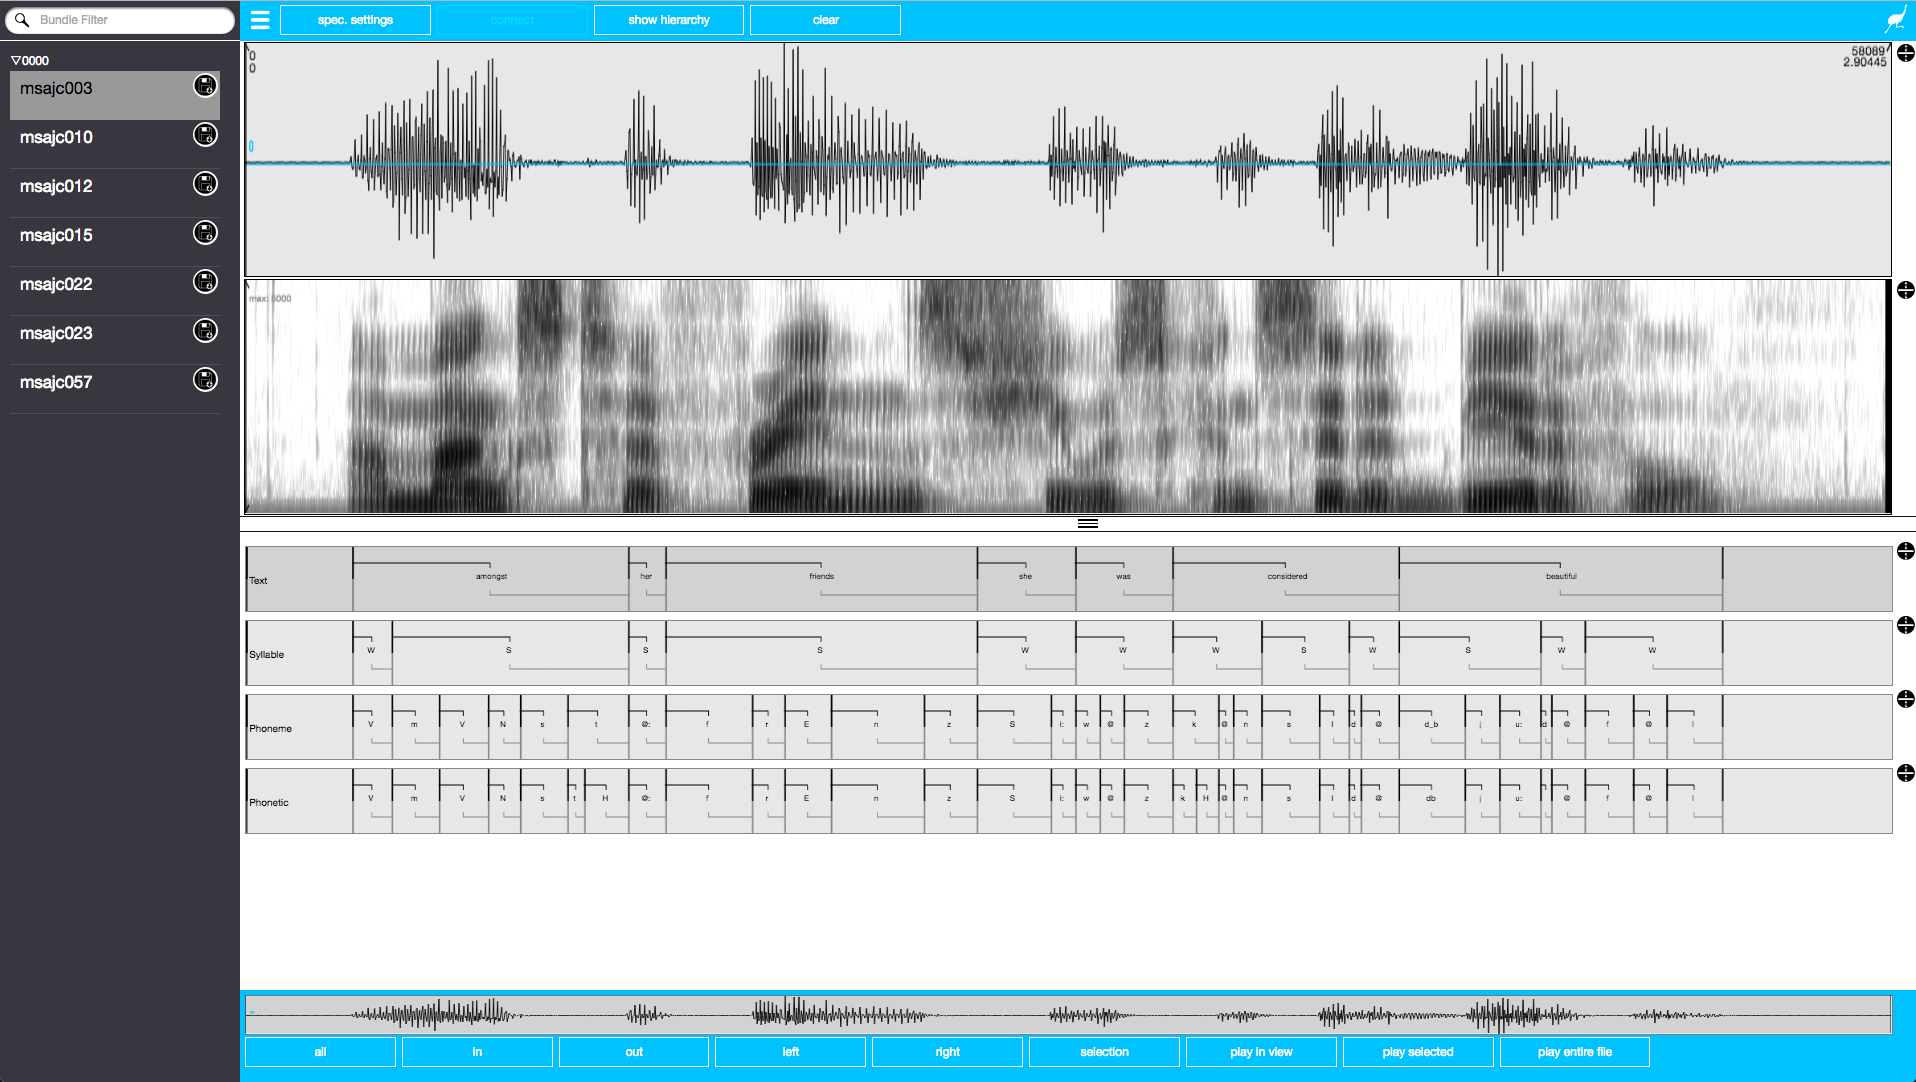
\includegraphics{pics/tutorialEmuWebAppMyFirst.png}
\caption{Screenshot of \texttt{EMU-webApp} displaying \texttt{msajc003}
bundle of \emph{myFirst}
\texttt{emuDB}.(\#fig:tutorial\_emuWebAppMyFirst)}
\end{figure}

\section{Querying and autobuilding the annotation
structure}\label{querying-and-autobuilding-the-annotation-structure}

An integral step in the default workflow of the EMU-SDMS is querying the
annotations of a database. The \texttt{emuDB} package implements a
\texttt{query()} function to accomplish this task. This function
evaluates an EMU Query Language (EQL) expression and extracts the
annotation items from the database that match a query expression. As
Chapter \ref{chap:querysys} gives a detailed description of the query
mechanics provided by \texttt{emuDB}, this tutorial will only use a very
small, hopefully easy to understand subset of the EQL.

The output of the \texttt{summary()} command in R Example
@ref(rexample:tutorial\_summary) and the screenshot in Figure
@ref(fig:tutorial\_emuWebAppMyFirst) show that the \emph{myFirst}
\texttt{emuDB} contains four levels of annotations. R Example
@ref(rexample:tutorial\_simpleQuery) shows four separate queries that
query various segments on each of the available levels. The query
expressions all use the matching operator \texttt{==} which returns
annotation items whose labels match those specified to the right of the
operator and that belong to the level specified to the left of the
operator (i.e., \texttt{LEVEL\ ==\ LABEL}; see Chapter
\ref{chap:querysys} for a detailed description).

\begin{Shaded}
\begin{Highlighting}[]
\CommentTok{# query all segments containing the label}
\CommentTok{# "was" of the "Phonetic" level}
\NormalTok{sl_text =}\StringTok{ }\KeywordTok{query}\NormalTok{(}\DataTypeTok{emuDBhandle =} \NormalTok{dbHandle,}
                \DataTypeTok{query =} \StringTok{"Text == was"}\NormalTok{)}

\CommentTok{# query all segments containing the label}
\CommentTok{# "S" (==strong syllable) of the "Syllable" level}
\NormalTok{sl_syl =}\StringTok{ }\KeywordTok{query}\NormalTok{(}\DataTypeTok{emuDBhandle =} \NormalTok{dbHandle,}
               \DataTypeTok{query =} \StringTok{"Syllable == S"}\NormalTok{)}

\CommentTok{# query all segments containing the label}
\CommentTok{# "n" on the "Phoneme" level}
\NormalTok{sl_phoneme =}\StringTok{ }\KeywordTok{query}\NormalTok{(dbHandle,}
                   \DataTypeTok{query =} \StringTok{"Phoneme == f"}\NormalTok{)}

\CommentTok{# query all segments containing the label}
\CommentTok{# "n" of the "Phonetic" level}
\NormalTok{sl_phonetic =}\StringTok{ }\KeywordTok{query}\NormalTok{(dbHandle,}
                    \DataTypeTok{query =} \StringTok{"Phonetic == n"}\NormalTok{)}

\CommentTok{# show class vector of query result}
\KeywordTok{class}\NormalTok{(sl_phonetic)}
\end{Highlighting}
\end{Shaded}

\begin{verbatim}
## [1] "emuRsegs"   "emusegs"    "data.frame"
\end{verbatim}

\begin{Shaded}
\begin{Highlighting}[]
\CommentTok{# show first entry of sl}
\KeywordTok{head}\NormalTok{(sl_phonetic, }\DataTypeTok{n =} \DecValTok{1}\NormalTok{)}
\end{Highlighting}
\end{Shaded}

\begin{verbatim}
## segment  list from database:  myFirst 
## query was:  Phonetic == n 
##   labels    start      end session   bundle    level    type
## 1      n 1031.925 1195.925    0000 msajc003 Phonetic SEGMENT
\end{verbatim}

\begin{Shaded}
\begin{Highlighting}[]
\CommentTok{# show summary of sl}
\KeywordTok{summary}\NormalTok{(sl_phonetic)}
\end{Highlighting}
\end{Shaded}

\begin{verbatim}
## segment  list from database:  myFirst 
## query was:  Phonetic == n 
##  with 12 segments
## 
## Segment distribution:
## 
##  n 
## 12
\end{verbatim}

As demonstrated in R Example @ref(rexample:tutorial\_simpleQuery), the
result of a query is an \texttt{emuRsegs} object, which is a super-class
of the common \texttt{data.frame}. This object is often referred to as a
segment list, or ``seglist''. A segment list carries information about
the extracted annotation items such as the extracted labels, the start
and end times of the segments, the sessions and bundles the items are
from and the levels they belong to. An in-depth description of the
information contained in a segment list is given in Section
@ref(sec:query\_emuRsegs). R Example
@ref(rexample:tutorial\_simpleQuery) shows that the \texttt{summary()}
function can also be applied to a segment list object to get an overview
of what is contained within it. This can be especially useful when
dealing with larger segment lists.

\subsection{Autobuilding}\label{autobuilding}

The simple queries illustrated above query segments from a single level
that match a certain label. However, the EMU-SDMS offers a mechanism for
performing inter-level queries such as: \emph{Query all Phonetic items
that contain the label ``n'' and are part of a strong syllable}. For
such queries to be possible, the EMU-SDMS offers very sophisticated
annotation structure modeling capabilities, which are described in
Chapter @ref(chap:annot\_struct\_mod). For the sake of this tutorial we
will focus on converting the flat segment level annotation structure
displayed in Figure @ref(fig:tutorial\_emuWebAppMyFirst) to a
hierarchical form as displayed in Figure
@ref(fig:tutorial\_violentlyHier), where only the \emph{Phonetic} level
carries time information and the annotation items on the other levels
are explicitly linked to each other to form a hierarchical annotation
structure.

\begin{figure}
\centering
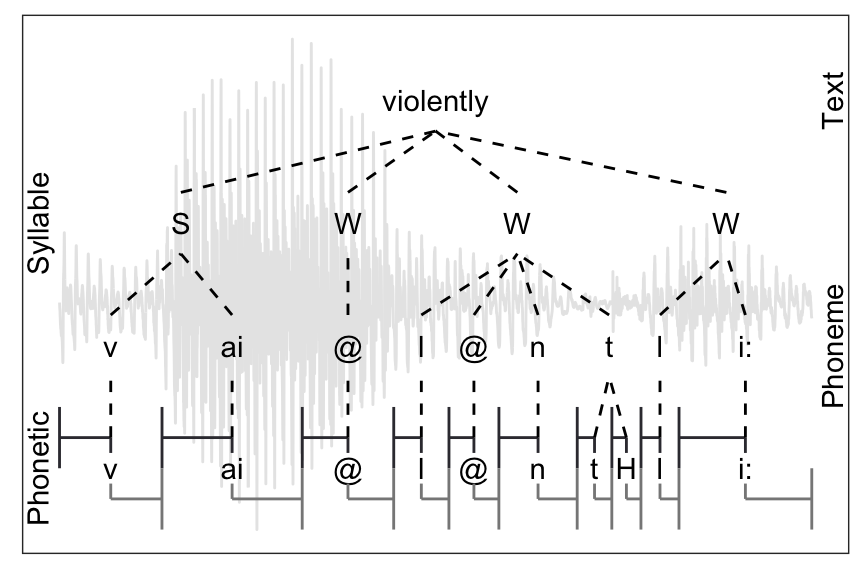
\includegraphics{The-EMU-SDMS-Manual_files/figure-latex/tutorial_violentlyHier-1.pdf}
\caption{(\#fig:tutorial\_violentlyHier)Example of a hierarchical
annotation of the word \emph{violently} belonging to the \emph{msajc012}
bundle of the \emph{myFirst} demo \texttt{emuDB}.}
\end{figure}

As it is a very laborious task to manually link annotation items
together using the \texttt{EMU-webApp} and the hierarchical information
is already implicitly contained in the time information of the segments
and events of each level, we will now use a simple function provided by
the \texttt{emuDB} package to build these hierarchical structures using
this information called \texttt{autobuild\_linkFromTimes()}. R Example
@ref(rexample:tutorial\_autobuild) shows the calls to this function
which autobuild the hierarchical annotations in the \emph{myFirst}
database. As a general rule for autobuilding hierarchical annotation
structures, a good strategy is to start the autobuilding process
beginning with coarser grained annotation levels (i.e., the
\emph{Text}/\emph{Syllable} level pair in our example) and work down to
finer grained annotations (i.e., the \emph{Syllable}/\emph{Phoneme} and
\emph{Phoneme}/\emph{Phonetic} level pairs in our example). To build
hierachical annotation structures we need link definitions, which
together with the level definitions define the annotation structure for
the entire database (see Chapter @ref(chap:annot\_struct\_mod) for
further details). The \texttt{autobuild\_linkFromTimes()} calls in R
Example @ref(rexample:tutorial\_autobuild) use the
\texttt{newLinkDefType} parameter, which if defined automatically adds a
link definition to the database.

\begin{Shaded}
\begin{Highlighting}[]
\CommentTok{# invoke autobuild function}
\CommentTok{# for "Text" and "Syllable" levels}
\KeywordTok{autobuild_linkFromTimes}\NormalTok{(dbHandle,}
                        \DataTypeTok{superlevelName =} \StringTok{"Text"}\NormalTok{,}
                        \DataTypeTok{sublevelName =} \StringTok{"Syllable"}\NormalTok{,}
                        \DataTypeTok{convertSuperlevel =} \OtherTok{TRUE}\NormalTok{,}
                        \DataTypeTok{newLinkDefType =} \StringTok{"ONE_TO_MANY"}\NormalTok{)}

\CommentTok{# invoke autobuild function}
\CommentTok{# for "Syllable" and "Phoneme" levels}
\KeywordTok{autobuild_linkFromTimes}\NormalTok{(dbHandle,}
                        \DataTypeTok{superlevelName =} \StringTok{"Syllable"}\NormalTok{,}
                        \DataTypeTok{sublevelName =} \StringTok{"Phoneme"}\NormalTok{,}
                        \DataTypeTok{convertSuperlevel =} \OtherTok{TRUE}\NormalTok{,}
                        \DataTypeTok{newLinkDefType =} \StringTok{"ONE_TO_MANY"}\NormalTok{)}

\CommentTok{# invoke autobuild function}
\CommentTok{# for "Phoneme" and "Phonetic" levels}
\KeywordTok{autobuild_linkFromTimes}\NormalTok{(dbHandle,}
                        \DataTypeTok{superlevelName =} \StringTok{"Phoneme"}\NormalTok{,}
                        \DataTypeTok{sublevelName =} \StringTok{"Phonetic"}\NormalTok{,}
                        \DataTypeTok{convertSuperlevel =} \OtherTok{TRUE}\NormalTok{,}
                        \DataTypeTok{newLinkDefType =} \StringTok{"MANY_TO_MANY"}\NormalTok{)}
\end{Highlighting}
\end{Shaded}

\begin{figure}
\centering
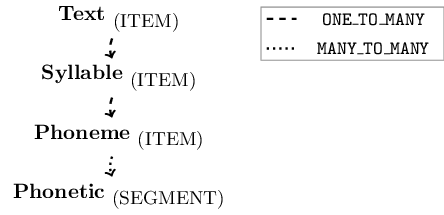
\includegraphics{pics/tut_simpleAnnotStruct.png}
\caption{Schematic annotation structure of the \texttt{emuDB} after
calling the autobuild function in R Example
@ref(rexample:tutorial\_autobuild).(\#fig:tutorial\_simpleAnnotStruct)}
\end{figure}

As the \texttt{autobuild\_linkFromTimes()} function automatically
creates backup levels to avoid the accidental loss of boundary or event
time information, R Example @ref(rexample:tutorial\_delBackupLevels)
shows how these backup levels can be removed to clean up the database.
However, using the \texttt{remove\_levelDefinition()} function with its
\texttt{force} parameter set to \texttt{TRUE} is a very invasive action.
Usually this would not be recommended, but for this tutorial we are
keeping everything as clean as possible.

\begin{Shaded}
\begin{Highlighting}[]
\CommentTok{# list level definitions}
\CommentTok{# as this reveals the "-autobuildBackup" levels}
\CommentTok{# added by the autobuild_linkFromTimes() calls}
\KeywordTok{list_levelDefinitions}\NormalTok{(dbHandle)}
\end{Highlighting}
\end{Shaded}

\begin{verbatim}
##                       name    type nrOfAttrDefs              attrDefNames
## 1                     Text    ITEM            1                     Text;
## 2                 Syllable    ITEM            1                 Syllable;
## 3                  Phoneme    ITEM            1                  Phoneme;
## 4                 Phonetic SEGMENT            1                 Phonetic;
## 5     Text-autobuildBackup SEGMENT            1     Text-autobuildBackup;
## 6 Syllable-autobuildBackup SEGMENT            1 Syllable-autobuildBackup;
## 7  Phoneme-autobuildBackup SEGMENT            1  Phoneme-autobuildBackup;
\end{verbatim}

\begin{Shaded}
\begin{Highlighting}[]
\CommentTok{# remove the levels containing the "-autobuildBackup"}
\CommentTok{# suffix}
\KeywordTok{remove_levelDefinition}\NormalTok{(dbHandle,}
                       \DataTypeTok{name =} \StringTok{"Text-autobuildBackup"}\NormalTok{,}
                       \DataTypeTok{force =} \OtherTok{TRUE}\NormalTok{,}
                       \DataTypeTok{verbose =} \OtherTok{FALSE}\NormalTok{)}

\KeywordTok{remove_levelDefinition}\NormalTok{(dbHandle,}
                       \DataTypeTok{name =} \StringTok{"Syllable-autobuildBackup"}\NormalTok{,}
                       \DataTypeTok{force =} \OtherTok{TRUE}\NormalTok{,}
                       \DataTypeTok{verbose =} \OtherTok{FALSE}\NormalTok{)}

\KeywordTok{remove_levelDefinition}\NormalTok{(dbHandle,}
                       \DataTypeTok{name =} \StringTok{"Phoneme-autobuildBackup"}\NormalTok{,}
                       \DataTypeTok{force =} \OtherTok{TRUE}\NormalTok{,}
                       \DataTypeTok{verbose =} \OtherTok{FALSE}\NormalTok{)}

\CommentTok{# list level definitions}
\KeywordTok{list_levelDefinitions}\NormalTok{(dbHandle)}
\end{Highlighting}
\end{Shaded}

\begin{verbatim}
##       name    type nrOfAttrDefs attrDefNames
## 1     Text    ITEM            1        Text;
## 2 Syllable    ITEM            1    Syllable;
## 3  Phoneme    ITEM            1     Phoneme;
## 4 Phonetic SEGMENT            1    Phonetic;
\end{verbatim}

\begin{Shaded}
\begin{Highlighting}[]
\CommentTok{# list level definitions}
\CommentTok{# which were added by the autobuild functions}
\KeywordTok{list_linkDefinitions}\NormalTok{(dbHandle)}
\end{Highlighting}
\end{Shaded}

\begin{verbatim}
##           type superlevelName sublevelName
## 1  ONE_TO_MANY           Text     Syllable
## 2  ONE_TO_MANY       Syllable      Phoneme
## 3 MANY_TO_MANY        Phoneme     Phonetic
\end{verbatim}

As can be seen by the output of \texttt{list\_levelDefinitions()} and
\textbackslash{} \texttt{list\_linkDefinitions()} in R Example
@ref(rexample:tutorial\_autobuild), the annotation structure of the
\emph{myFirst} \texttt{emuDB} now matches that displayed in Figure
@ref(fig:tutorial\_simpleAnnotStruct). Using the \texttt{serve()}
function to open the \texttt{emuDB} in the \texttt{EMU-webApp} followed
by clicking on the \texttt{show\ hierarchy} button in the top menu (and
rotating the hierarchy by 90 degrees by clicking the
\texttt{rotate\ by\ 90\ degrees} button) will result in a view similar
to the screenshot of Figure
@ref(fig:tutorial\_EMU-webAppScreenshotTutorialPostAutobHier).

\begin{figure}
\centering
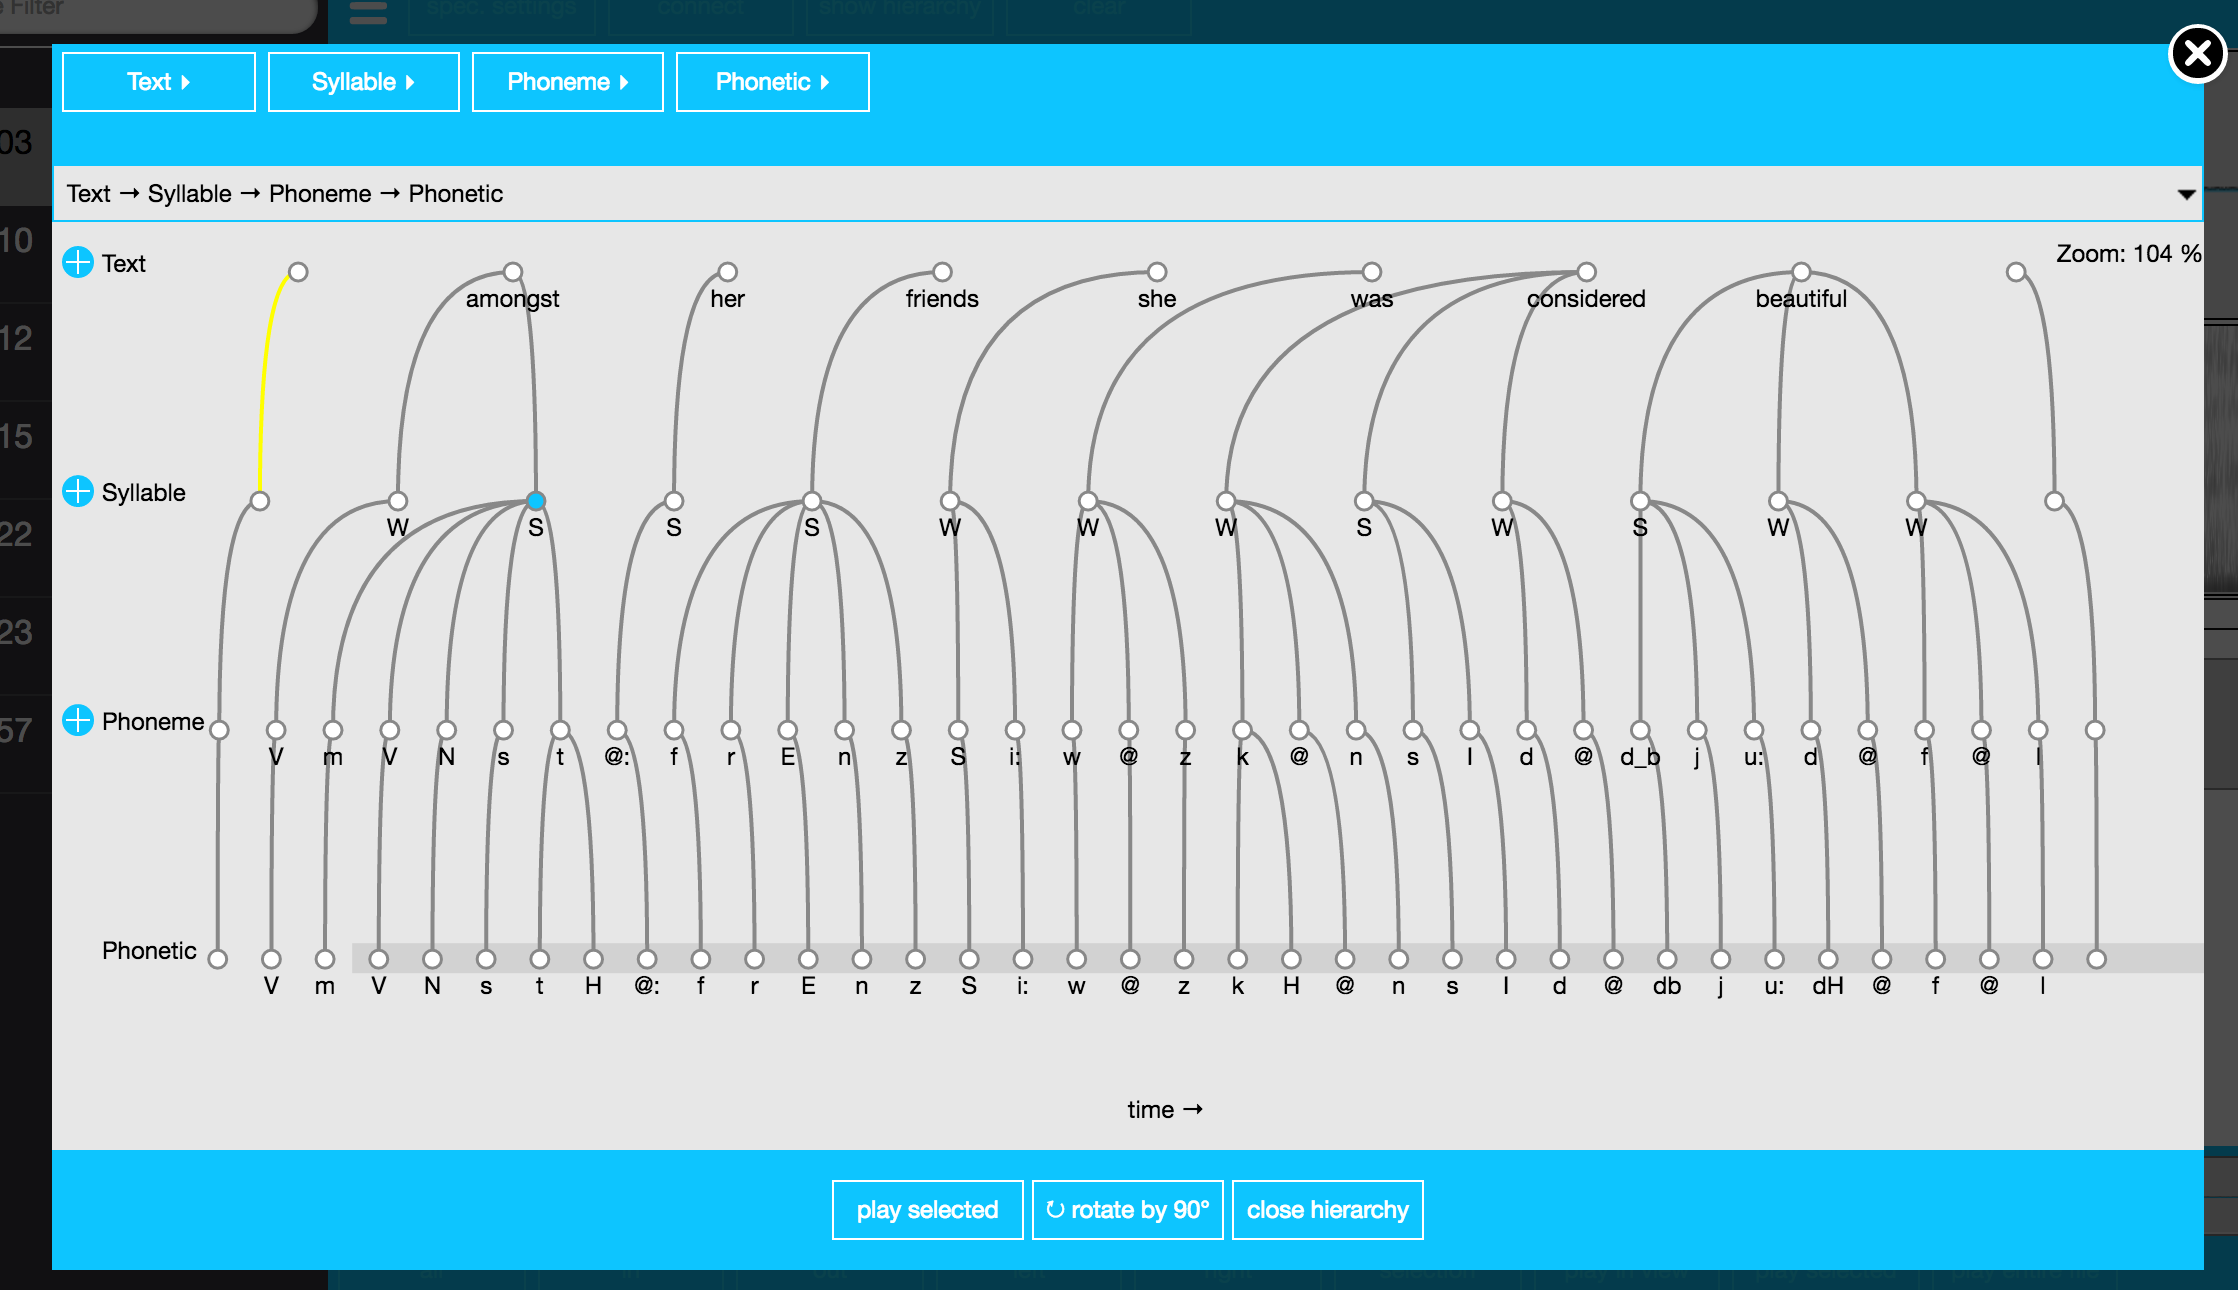
\includegraphics{pics/EMU-webAppScreenshotTutorialPostAutobHier.png}
\caption{Screenshot of \texttt{EMU-webApp} displaying the autobuilt
hierarchy of the \emph{myFirst}
\texttt{emuDB}.(\#fig:tutorial\_EMU-webAppScreenshotTutorialPostAutobHier)}
\end{figure}

\subsection{Querying the hierarchical
annotations}\label{querying-the-hierarchical-annotations}

Having this hierarchical annotation structure now allows us to formulate
a query that helps answer the originally stated question: \emph{Given an
annotated speech database, is vowel height (measured by its correlate,
the first formant frequency) influenced by whether it appears in a
strong or weak syllable?}. As stated in the question, we are interested
in all the vowels in our database. R Example
@ref(rexample:tutorial\_labelGroupQuery) shows how all the vowels in the
\emph{myFirst} database are queried.

\begin{Shaded}
\begin{Highlighting}[]
\CommentTok{# query the label group on the Phonetic level}
\CommentTok{# Note that the use of paste0() is optional, as}
\CommentTok{# it is only used for formatting purposes}
\NormalTok{sl_vowels =}\StringTok{ }\KeywordTok{query}\NormalTok{(dbHandle, }\KeywordTok{paste0}\NormalTok{(}\StringTok{"Phonetic == A | E | EC "}\NormalTok{,}
                                   \StringTok{"| I | V | U | ai | ei | oi "}\NormalTok{,}
                                   \StringTok{"| i@ | u@ | au | @u | @: "}\NormalTok{,}
                                   \StringTok{"| @ | '=' | a: | e: | i: "}\NormalTok{,}
                                   \StringTok{"| o: | u:"}\NormalTok{))}

\CommentTok{# show first entry of sl}
\KeywordTok{head}\NormalTok{(sl_vowels, }\DataTypeTok{n =} \DecValTok{1}\NormalTok{)}
\end{Highlighting}
\end{Shaded}

\begin{verbatim}
## segment  list from database:  myFirst 
## query was:  Phonetic == A | E | EC | I | V | U | ai | ei | oi | i@ | u@ | au | @u | @: | @ | ''='' | a: | e: | i: | o: | u: 
##   labels   start     end session   bundle    level    type
## 1      V 187.425 256.925    0000 msajc003 Phonetic SEGMENT
\end{verbatim}

As the type of syllable (strong vs.~week) for each vowel that was just
extracted is also needed, we can use the requery functionality of the
EMU-SDMS (see Chapter \ref{chap:querysys}) to retrieve the syllable type
for each vowel. A requery essentially moves through a hierarchical
annotation (vertically or horizontally) starting from the segments that
are passed into the requery function. R Example
@ref(rexample:tutorial\_requery) illustrates the usage of the
hierarchical requery function, \texttt{requery\_hier()}, to retrieve the
appropriate annotation items from the \emph{Syllable} level.

\begin{Shaded}
\begin{Highlighting}[]
\CommentTok{# hierarchical requery starting from the items in sl_vowels}
\CommentTok{# and moving up to the "Syllable" level}
\NormalTok{sl_sylType =}\StringTok{ }\KeywordTok{requery_hier}\NormalTok{(dbHandle,}
                          \DataTypeTok{seglist =} \NormalTok{sl_vowels,}
                          \DataTypeTok{level =} \StringTok{"Syllable"}\NormalTok{,}
                          \DataTypeTok{calcTimes =} \OtherTok{FALSE}\NormalTok{)}

\CommentTok{# show first entry of sl}
\KeywordTok{head}\NormalTok{(sl_sylType, }\DataTypeTok{n =} \DecValTok{1}\NormalTok{)}
\end{Highlighting}
\end{Shaded}

\begin{verbatim}
## segment  list from database:  myFirst 
## query was:  FROM REQUERY 
##   labels start end session   bundle    level type
## 1      W    NA  NA    0000 msajc003 Syllable ITEM
\end{verbatim}

\begin{Shaded}
\begin{Highlighting}[]
\CommentTok{# show that sl_vowel and sl_sylType have the}
\CommentTok{# same number of row entries}
\KeywordTok{nrow}\NormalTok{(sl_vowels) ==}\StringTok{ }\KeywordTok{nrow}\NormalTok{(sl_sylType)}
\end{Highlighting}
\end{Shaded}

\begin{verbatim}
## [1] TRUE
\end{verbatim}

As can be seen by the \texttt{nrow()} comparison in R Example
@ref(rexample:tutorial\_requery), the segment list returned by the
\texttt{requery\_hier()} function has the same number of rows as the
original \texttt{sl\_vowels} segment list. This is important, as each
row of both segment lists line up and allow us to infer which segment
belongs to which syllable (e.g., vowel \texttt{sl\_vowels{[}5,{]}}
belongs to syllable \texttt{sl\_sylType{[}5,{]}}).

\section{Signal extraction and
exploration}\label{section:tutorial_sigExtrAndExpl}

Now that the vowel and syllable type information including the vowel
start and end time information has been extracted from the database,
this information can be used to extract signal data that matches these
segments. Using the \texttt{emuDB} function \texttt{get\_trackdata()} we
can calculate the formant values in real time using the formant
estimation function, \texttt{forest()}, provided by the \texttt{wrassp}
package (see Chapter \ref{chap:wrassp} for details). R Example
@ref(rexample:tutorial\_getTrackdata) shows the usage of this function.

\begin{Shaded}
\begin{Highlighting}[]
\CommentTok{# get formant values for}
\NormalTok{td_vowels =}\StringTok{ }\KeywordTok{get_trackdata}\NormalTok{(dbHandle,}
                          \DataTypeTok{seglist =} \NormalTok{sl_vowels,}
                          \DataTypeTok{onTheFlyFunctionName =} \StringTok{"forest"}\NormalTok{,}
                          \DataTypeTok{verbose =} \NormalTok{F)}

\CommentTok{# show class vector}
\KeywordTok{class}\NormalTok{(td_vowels)}
\end{Highlighting}
\end{Shaded}

\begin{verbatim}
## [1] "trackdata"
\end{verbatim}

\begin{Shaded}
\begin{Highlighting}[]
\CommentTok{# show dimensions}
\KeywordTok{dim}\NormalTok{(td_vowels)}
\end{Highlighting}
\end{Shaded}

\begin{verbatim}
## [1] 81  4
\end{verbatim}

\begin{Shaded}
\begin{Highlighting}[]
\CommentTok{# display all values for fifth segment}
\NormalTok{td_vowels[}\DecValTok{5}\NormalTok{,]}
\end{Highlighting}
\end{Shaded}

\begin{verbatim}
## trackdata from track: fm 
## index:
##  left right
##     1     9
## ftime:
##       start    end
## [1,] 1422.5 1462.5
## data:
##         T1   T2   T3   T4
## 1422.5 297 2041 2470 3383
## 1427.5 290 2034 2409 3380
## 1432.5 288 2044 2277 3380
## 1437.5 288 1998 2143 3347
## 1442.5 287 1727 2138 3315
## 1447.5 287 1633 2119 3338
## 1452.5 295 1600 2114 3361
## 1457.5 292 1478 2112 3383
## 1462.5 290 1339 2071 3372
\end{verbatim}

As can be seen by the call to the \texttt{class()} function, the
resulting object is of the type \texttt{trackdata} and has 81 entries.
This corresponds to the number of rows contained in the segment lists
extracted above (i.e., \texttt{nrow(sl\_vowels)}). This indicates that
this object contains data for each of the segments that correspond to
each of the row entries of the segment lists (i.e.,
\texttt{td\_vowels{[}5,{]}} are the formant values belonging to
\texttt{sl\_vowels{[}5,{]}}). As the columns \texttt{T1}, \texttt{T2},
\texttt{T3}, \texttt{T4} of the printed output of
\texttt{td\_vowels{[}5,{]}} suggest, the \texttt{forest} function
estimates four formant values. We will only be concerned with the first
(column \texttt{T1}) and second (column \texttt{T2}). R Example
@ref(rexample:tutorial\_dplot) shows a call to \texttt{emuDB}'s
\texttt{dplot()} function which produces the plot displayed in Figure
@ref(fig:tutorial\_dplot). The first call to the \texttt{dplot()}
function plots all 81 first formant trajectories (achieved by indexing
the first column i.e., \texttt{T1}:
\texttt{x\ =\ td\_vowels{[},\ 1{]}}). The 81 trajectories are color
coded by vowel label
(\texttt{labs\ =\ sl\_vowels\textbackslash{}\$labels}). To clean up the
cluttered left plot, the second call to the \texttt{dplot()} function
additionally uses the \texttt{average} parameter to plot only the
ensemble averages of each vowel label and time-normalizes the
trajectories (\texttt{normalise\ =\ TRUE}) to an interval between 0 and
1.

\begin{Shaded}
\begin{Highlighting}[]
\CommentTok{# two plots next to each other}
\KeywordTok{par}\NormalTok{(}\DataTypeTok{mfrow =} \KeywordTok{c}\NormalTok{(}\DecValTok{1}\NormalTok{,}\DecValTok{2}\NormalTok{))}

\KeywordTok{dplot}\NormalTok{(}\DataTypeTok{x =} \NormalTok{td_vowels[, }\DecValTok{1}\NormalTok{],}
      \DataTypeTok{labs =} \NormalTok{sl_vowels$labels,}
      \DataTypeTok{xlab =} \StringTok{"Duration (ms)"}\NormalTok{,}
      \DataTypeTok{ylab =} \StringTok{"F1 (Hz)"}\NormalTok{)}

\KeywordTok{dplot}\NormalTok{(}\DataTypeTok{x =} \NormalTok{td_vowels[, }\DecValTok{1}\NormalTok{],}
      \DataTypeTok{labs =} \NormalTok{sl_vowels$labels,}
      \DataTypeTok{normalise =} \OtherTok{TRUE}\NormalTok{,}
      \DataTypeTok{average =} \OtherTok{TRUE}\NormalTok{,}
      \DataTypeTok{xlab =} \StringTok{"Normalized time"}\NormalTok{,}
      \DataTypeTok{ylab =} \StringTok{"F1 (Hz)"}\NormalTok{)}

\CommentTok{# back to single plot}
\KeywordTok{par}\NormalTok{(}\DataTypeTok{mfrow =} \KeywordTok{c}\NormalTok{(}\DecValTok{1}\NormalTok{,}\DecValTok{1}\NormalTok{))}
\end{Highlighting}
\end{Shaded}

\begin{figure}
\centering
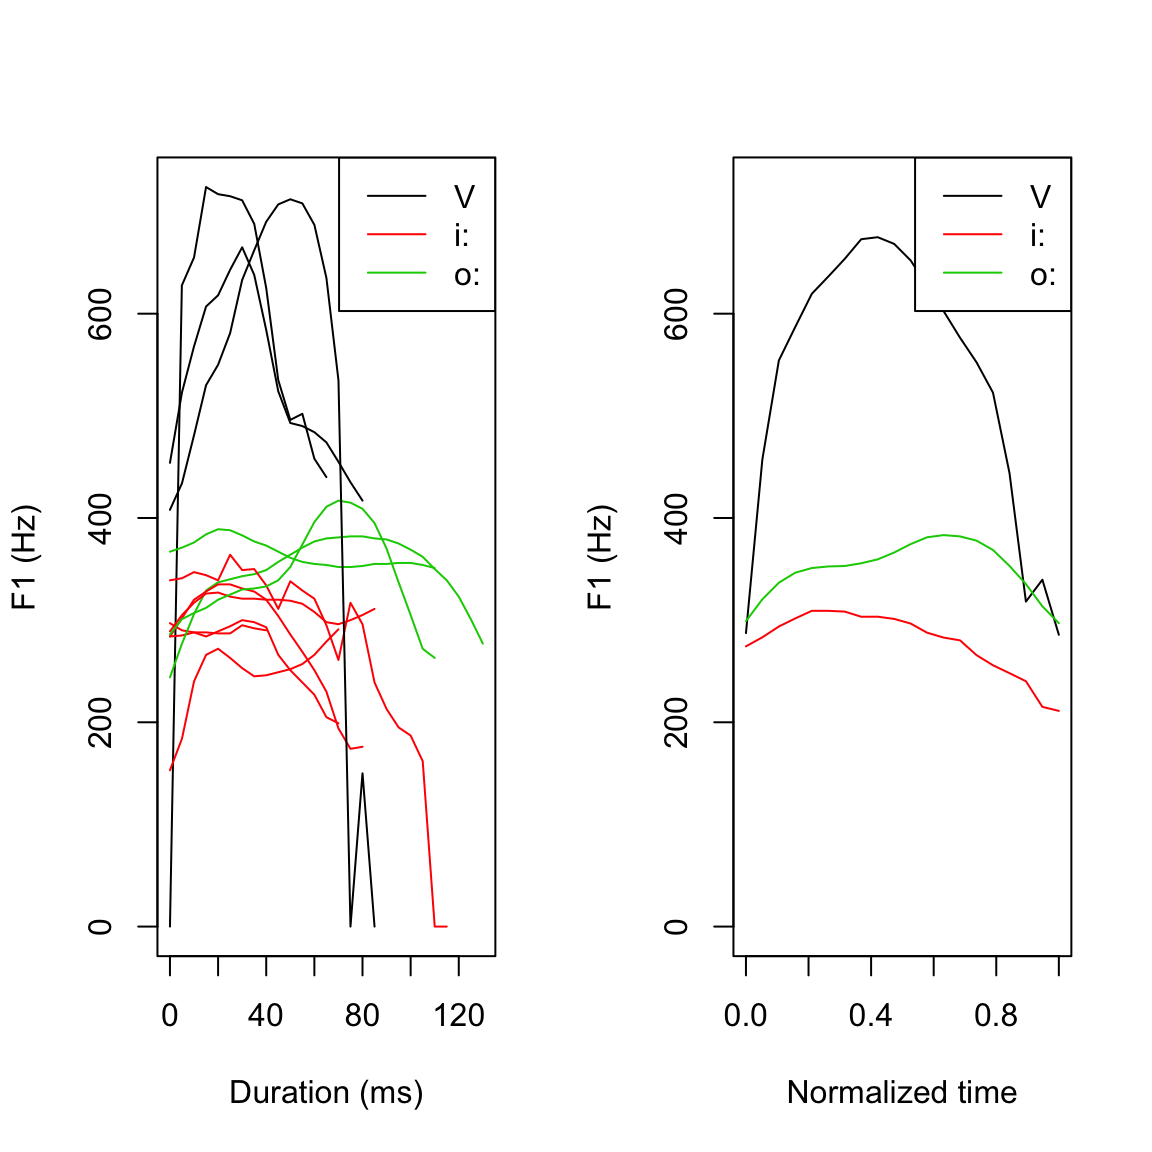
\includegraphics{The-EMU-SDMS-Manual_files/figure-latex/tutorial_dplot-1.pdf}
\caption{(\#fig:tutorial\_dplot)\texttt{dplot()} plots of F1
trajectories. The left plot displays 81 trajectories while the right
plot displays ensemble averages of each vowel.}
\end{figure}

Figure @ref(fig:tutorial\_dplot) gives an overview of the second formant
trajectories by vowel class. For the purpose of data exploration and to
get an idea of where the individual vowel classes lie on the F2 x F1
plane, which indirectly provides information about vowel height and
tongue position, R Example @ref(rexample:tutorial\_eplot) makes use of
the \texttt{eplot()} function. This produces Figure
@ref(fig:tutorial\_eplot). To be able to use the \texttt{eplot()}
function, the \texttt{td\_vowels} object first has to be modified, as it
contains entire formant trajectories but two dimensional data is needed
to be able to display it on the F2 x F1 plain. This can, for example, be
achieved by only extracting temporal mid-point formant values for each
vowel using the \texttt{get\_trackdata()} function utilizing its
\texttt{cut} parameter. R Example @ref(rexample:tutorial\_eplot) shows
an alternative approach using the \texttt{dcut()} function to
essentially cut the formant trajectories to a specified proportional
segment. By using only the \texttt{left.time\ =\ 0.5} (and not
specifying \texttt{right.time}) only the formant values that are closest
to the temporal mid-point are cut from the trajectories.

\begin{Shaded}
\begin{Highlighting}[]
\CommentTok{# cut formant trajectories at temporal mid-point}
\NormalTok{td_vowels_midpoint =}\StringTok{ }\KeywordTok{dcut}\NormalTok{(td_vowels,}
                          \DataTypeTok{left.time =} \FloatTok{0.5}\NormalTok{,}
                          \DataTypeTok{prop =} \OtherTok{TRUE}\NormalTok{)}

\CommentTok{# show dimensions of td_vowels_midpoint}
\KeywordTok{dim}\NormalTok{(td_vowels_midpoint)}

\CommentTok{# generate plot}
\KeywordTok{eplot}\NormalTok{(}\DataTypeTok{x =} \NormalTok{td_vowels_midpoint[,}\DecValTok{1}\NormalTok{:}\DecValTok{2}\NormalTok{],}
      \DataTypeTok{labs =} \NormalTok{sl_vowels$labels,}
      \DataTypeTok{dopoints =} \OtherTok{TRUE}\NormalTok{,}
      \DataTypeTok{xlab=}\StringTok{"F2 (Hz)"}\NormalTok{,}
      \DataTypeTok{ylab =} \StringTok{"F1 (Hz)"}\NormalTok{)}
\end{Highlighting}
\end{Shaded}

\begin{figure}
\centering
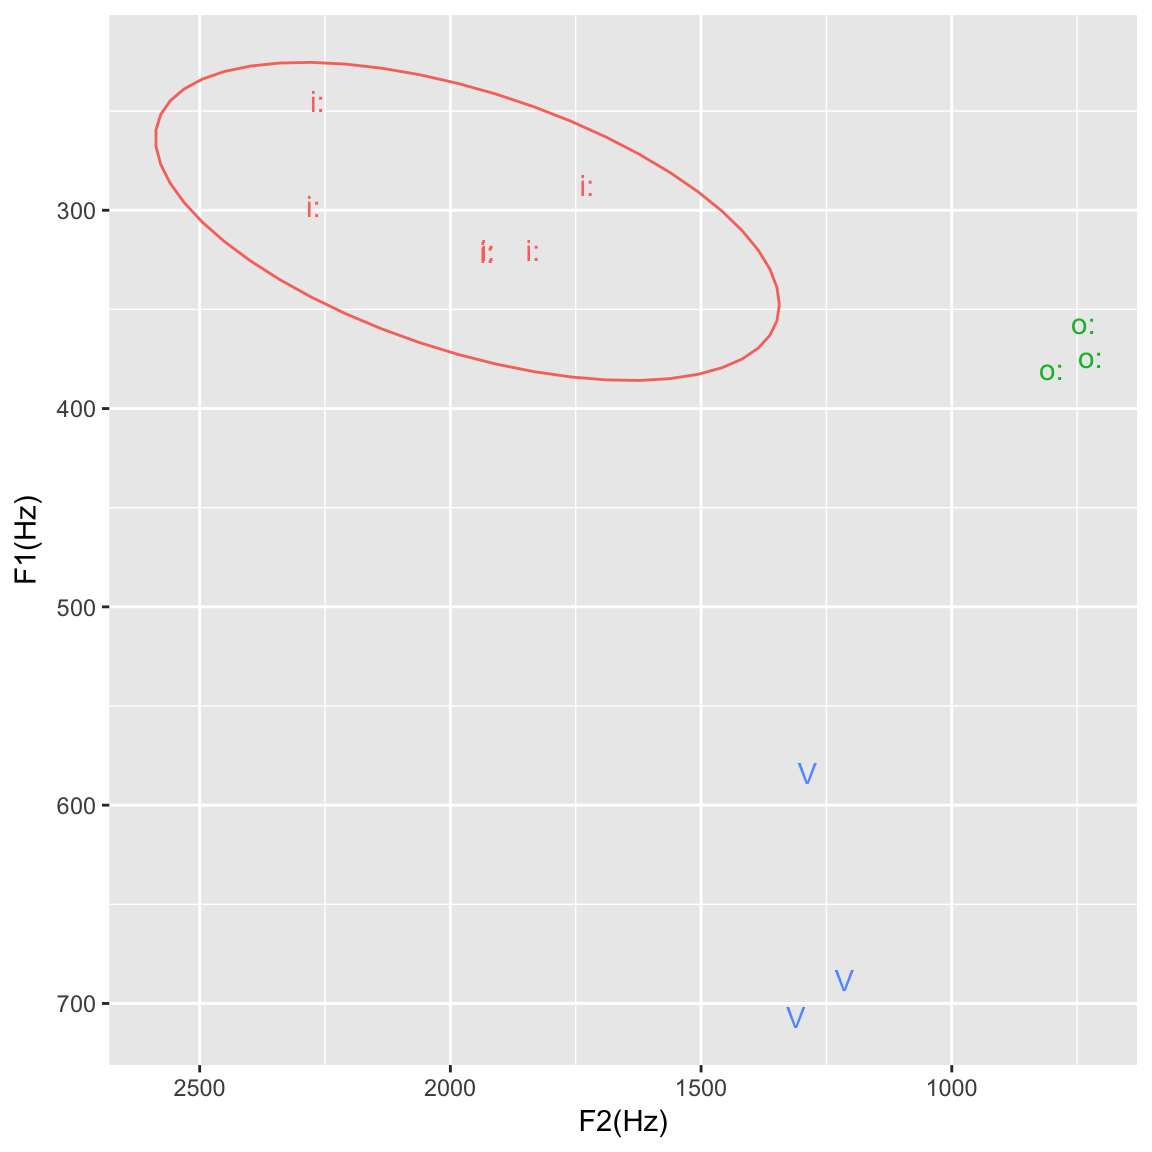
\includegraphics{The-EMU-SDMS-Manual_files/figure-latex/tutorial_eplot-1.pdf}
\caption{(\#fig:tutorial\_eplot)95\% ellipses for F2 x F1 data extracted
from the temporal midpoint separated by vowel.}
\end{figure}

Figure @ref(fig:tutorial\_eplot) displays the first two formants
extracted at the temporal midpoint of every vowel in
\texttt{sl\_vowels}. These formants are plotted on the F2 x F1 plane,
and their 95\% ellipsis distributions are also shown. Although not
necessarily applicable to the question posed at the beginning of this
tutorial, the data exploration using the \texttt{dplot()} and
\texttt{eplot()} functions can be very helpful tools for providing an
overview of the data at hand.

\section{Conclusion}\label{conclusion}

The tutorial given in this chapter gave an overview of what it is like
working with the EMU-SDMS to try to solve a research question. As many
of the concepts were only briefly explained, it is worth noting that
explicit explanations of the various components and integral concepts
are given in following chapters. Further, additional use cases that have
been taken from the \texttt{emuR\_intro} vignette can be found in
Appendix @ref(app\_chap:useCases). These use cases act as templates for
various types of research questions and will hopefully aid the user in
finding a solution similar to what she or he wishes to achieve.

\chapter{The query system}\label{the-query-system}

\chapter{Toolchain SpeechRecorder --- MAUS ---
EMU-SDMS}\label{toolchain-speechrecorder-maus-emu-sdms}

Most phonetic research projects involve this workflow:

\begin{enumerate}
\def\labelenumi{\arabic{enumi}.}
\tightlist
\item
  Record speech
\item
  Annotate speech using automatic tools
\item
  Check and correct the generated annotations by hand
\item
  Analyze speech (connecting the primary data with annotations and
  derived signals)
\end{enumerate}

The EMU Speech Database Management System is focused on steps 3 and 4 of
this workflow. For the first two steps, it can very usefully be
complemented by two other tools:
\href{http://www.speechrecorder.org/}{SpeechRecorder} and MAUS (or, more
broadly speaking --- and more correctly, for that matter --- the
\href{https://clarin.phonetik.uni-muenchen.de/BASWebServices}{BAS Web
Services}). This chapter introduces how the tools can be combined --- in
a systematic way, with as little fuss as possible.

\section{What do SpeechRecorder and MAUS
do?}\label{what-do-speechrecorder-and-maus-do}

``SpeechRecorder is a platform independent audio recording software
customized to the requirements of speech recordings''
(\url{http://www.speechrecorder.org/}). To this end, SpeechRecorder lets
you define prompts that participants will read (or otherwise react to)
while you are recording them. At the end of a session, instead of one
large recording of the whole session, you have a set of smaller audio
recordings, each one representing a single prompt.

MAUS (Munich AUtomatic Segmentation) processes audio recordings with
corresponding orthographic transcriptions, and outputs (1) a
corresponding phonetic transcription and (2) a segmentation of the
signal into individual speech sounds. As such, MAUS is a part of the
\href{https://clarin.phonetik.uni-muenchen.de/BASWebServices}{BAS Web
Services}. \footnote{Strictly speaking, MAUS is used in conjunction with
  G2P and possibly Chunker to achieve this result. The whole package is
  often referred to as MAUS, however.}

\section{Different types of prompts}\label{different-types-of-prompts}

Prompts are very often sentences that participants read out aloud
(producing \emph{read speech}). However, this need not be the case.
Prompts may as well be, for example, images that participants have to
name or describe, or written questions that participants answer.

In terms of processing, \emph{read speech} has the advantage that the
researcher already has orthographic transcriptions of all recordings,
because the prompts \emph{are} the transcriptions (this neglects
hesitations, misread utterances, etc.).

For all cases besides read speech, transcriptions have to be prepared.
For read speech, when hesitations etc. need to be considered, the
existing transcriptions need to be corrected (per token). For the time
being, this is out of the scope of this book.\footnote{It will be
  covered, at a later time, in this or a separate chapter.}

\section{Combining the tools}\label{combining-the-tools}

The order of the processing steps is unchangeable: The files have to be
recorded first, then annotated and then analyzed.

However, there are different ways of passing data around between the
tools. For example SpeechRecorder might \emph{export} files into emuDB
format or the EMU-SDMS might \emph{import} files stored in
SpeechRecorder's format. After all, they are separate tools and can be
used individually (although the combination makes great sense).

Moreover, sometimes a database grows, and some new files are recorded
while others have already been annotated or analyzed (which challenges
the ``unchangeable order of processing steps'').

We can see now that we have to convert our data between different
formats. We want to benefit from all tools but keep the conversion work
down to a minimum. In this section, we explain the (currently) best way
to do this. We will import SpeechRecorder's recordings and prompts into
the EMU-SDMS and then use emuR to send the data to MAUS and other BAS
Web Services.

\subsection{Importing recordings and transcriptions into
Emu}\label{importing-recordings-and-transcriptions-into-emu}

\subsubsection{Using the import\_speechRecorder()
function}\label{using-the-import_speechrecorder-function}

The \texttt{import\_speechRecorder()} function is in the making, but
unfortunately not finished yet. We therefore have to resort to the
second-best way of importing SpeechRecorder's results into Emu:

\subsubsection{Using intermediary text
files}\label{using-intermediary-text-files}

SpeechRecorder, per default, saves one .wav file for each prompt. With
additional settings, it will save a .txt file containing the
corresponding prompt along with each .wav file. This is great because it
is exactly what MAUS needs as its input.

The following options must be configured \emph{before recordings are
made}. Note that parts of SpeechRecorder's user interface are in German:

\begin{itemize}
\tightlist
\item
  Under ``Projekt / Einstellungen\ldots{} / Annotation'':

  \begin{itemize}
  \tightlist
  \item
    Under ``Persist'', tick the checkbox that says ``Simple text loader
    writer for annotation template for MAUS processing''
  \item
    Under ``Auto annotation'', tick the checkbox that says ``Prompt
    template auto annotator'' (note that the two checkboxes are very
    similar. Make sure to tick the right one.)
  \end{itemize}
\item
  In your script:

  \begin{itemize}
  \tightlist
  \item
    If you edit the XML file directly: Make sure each of your
    \texttt{\textless{}mediaitem\textgreater{}} elements has the
    attribute \texttt{annotationTemplate="true"}
  \item
    If you use the integrated script editor: Make sure to tick the
    checkbox ``Use as annotation template'' for \emph{every recording}.
  \end{itemize}
\end{itemize}

Now, after your recording session, you will have audio and text files.
In emuR, this combination is called a \emph{txt collection}. We will
thus use the function \texttt{convert\_txtCollection}, to import
SpeechRecorder's files into Emu's format. In the following example, we
will use the sample txt collection included with the emuR package.

\begin{Shaded}
\begin{Highlighting}[]
\CommentTok{# Load the emuR package}
\KeywordTok{library}\NormalTok{(emuR)}

\CommentTok{# Create demo data in directory provided by tempdir()}
\KeywordTok{create_emuRdemoData}\NormalTok{(}\DataTypeTok{dir =} \KeywordTok{tempdir}\NormalTok{())}

\CommentTok{# Import the sample txt collection.}
\CommentTok{# When used with real data, sourceDir should point to the RECS directory of your}
\CommentTok{# SpeechRecorder project.}
\KeywordTok{convert_txtCollection}\NormalTok{(}\DataTypeTok{dbName =} \StringTok{"myEmuDatabase"}\NormalTok{,}
                      \DataTypeTok{sourceDir =} \KeywordTok{file.path}\NormalTok{(}\KeywordTok{tempdir}\NormalTok{(), }\StringTok{"emuR_demoData"}\NormalTok{, }\StringTok{"txt_collection"}\NormalTok{),}
                      \DataTypeTok{targetDir =} \KeywordTok{tempdir}\NormalTok{())}

\NormalTok{dbHandle =}\StringTok{ }\KeywordTok{load_emuDB}\NormalTok{(}\KeywordTok{file.path}\NormalTok{(}\KeywordTok{tempdir}\NormalTok{(), }\StringTok{"myEmuDatabase_emuDB"}\NormalTok{))}
\end{Highlighting}
\end{Shaded}

Now, you have an Emu database. You can inspect it using

\begin{Shaded}
\begin{Highlighting}[]
\KeywordTok{summary}\NormalTok{(dbHandle)}
\end{Highlighting}
\end{Shaded}

or

\begin{Shaded}
\begin{Highlighting}[]
\KeywordTok{serve}\NormalTok{(dbHandle)}
\end{Highlighting}
\end{Shaded}

The database contains all our recordings, and exactly one type of
annotation: orthographic transcription. No phonetic transcription, no
segmentation. The next section will cover that.

\subsection{Feeding the data into
MAUS}\label{feeding-the-data-into-maus}

The .wav and .txt files could have been uploaded on the
\href{https://clarin.phonetik.uni-muenchen.de/BASWebServices/\#!/services/Pipeline}{BAS
web site}, but we will do it using emuR. This is generally less
error-prone and requires less manual work. Moreover, since it is a
scripted way of doing things, we can reproduce it reliably.

To process the data, we make use of several of emuR's functions called
\texttt{runBASwebservice\_...}. They will upload the data to WebMAUS and
accompanying services and save the results directly inside your existing
emuDB (this of course takes some time, depending on the size of your
database and the speed of your internet connection).

\begin{Shaded}
\begin{Highlighting}[]
\KeywordTok{runBASwebservice_g2pForTokenization}\NormalTok{(}\DataTypeTok{handle =} \NormalTok{dbHandle,}
                                    \DataTypeTok{language =} \StringTok{"eng-US"}\NormalTok{,}
                                    \DataTypeTok{transcriptionAttributeDefinitionName =} \StringTok{"transcription"}\NormalTok{,}
                                    \DataTypeTok{orthoAttributeDefinitionName =} \StringTok{"Word"}\NormalTok{)}

\KeywordTok{runBASwebservice_g2pForPronunciation}\NormalTok{(}\DataTypeTok{handle =} \NormalTok{dbHandle,}
                                     \DataTypeTok{language =} \StringTok{"eng-US"}\NormalTok{,}
                                     \DataTypeTok{orthoAttributeDefinitionName =} \StringTok{"Word"}\NormalTok{,}
                                     \DataTypeTok{canoAttributeDefinitionName =} \StringTok{"Canonical"}\NormalTok{)}

\KeywordTok{runBASwebservice_maus}\NormalTok{(}\DataTypeTok{handle =} \NormalTok{dbHandle,}
                      \DataTypeTok{language =} \StringTok{"eng-US"}\NormalTok{,}
                      \DataTypeTok{canoAttributeDefinitionName =} \StringTok{"Canonical"}\NormalTok{,}
                      \DataTypeTok{mausAttributeDefinitionName =} \StringTok{"Phonetic"}\NormalTok{)}
\end{Highlighting}
\end{Shaded}

When the services are finished, we can use

\begin{Shaded}
\begin{Highlighting}[]
\KeywordTok{serve}\NormalTok{(db)}
\end{Highlighting}
\end{Shaded}

to inspect the database with the new annotations. This time, it includes
segmentation into words and phonemes, canonical phonetic transcription
and realized phonetic transcription.

This chapter described the current best practice of combining
SpeechRecorder, MAUS and the EMU-SDMS to fit a typical phonetic project
workflow.

\bibliography{packages.bib,book.bib}


\end{document}
